\documentclass[12pt]{article}

% Language setting
% Replace `english' with e.g. `spanish' to change the document language
\usepackage[english]{babel}

% Set page size and margins
% Replace `letterpaper' with `a4paper' for UK/EU standard size
\usepackage[letterpaper,top=2cm,bottom=2cm,left=3cm,right=3cm,marginparwidth=1.75cm]{geometry}

% Useful packages
\usepackage{xcolor} % For color in the text
\definecolor{astana}{RGB}{220,220,220}
\definecolor{gray}{RGB}{128,128,128}
\definecolor{red}{RGB}{255,0,0}
\usepackage{makecell}
\usepackage{multirow}
\usepackage{amsmath} % For math
\usepackage{subcaption} % For subfigures
\usepackage{fancyhdr}
\usepackage{amsmath}
\usepackage{graphicx}
\usepackage[colorlinks=true, allcolors=blue]{hyperref}
\usepackage{titlesec}
\usepackage{enumitem}
\usepackage{amssymb}
\usepackage{amsthm}
\usepackage{tikz}
\usepackage{pgfplots}
\usepackage{float}
\usepackage{subcaption}
\usepackage{listings}
\usepackage{color}
\usepackage{listings}
% Define custom colors for code highlighting
\definecolor{codebackground}{RGB}{255,253,238}  % Light yellow
\definecolor{codecomment}{RGB}{0,128,0}        % Dark green
\definecolor{codekeyword}{RGB}{0,0,255}         % Blue
\definecolor{codenumber}{RGB}{128,128,128}      % Gray
\definecolor{codestring}{RGB}{189, 36, 209}           % Violet
\definecolor{codecyan}{RGB}{0,255,255}           % Cyan
\definecolor{codeorange}{RGB}{255,165,0}         % Orange
\definecolor{codepurple}{RGB}{128,0,128}         % Purple
% Set the code style
\lstdefinestyle{mystyle}{
    language=Python,
    basicstyle=\small\ttfamily,
    commentstyle=\color{codecomment},
    keywordstyle=\color{codekeyword},
    numberstyle=\tiny\color{codenumber},
    stringstyle=\color{codestring},
    morekeywords={as},
    emph={True, False, None},
    emphstyle=\color{codepurple},
    backgroundcolor=\color{codebackground},
    breaklines=true,
    showtabs=false,
    showspaces=false,
    numbers=left,
    frame=single,
    captionpos=b,
    tabsize=2
}
% 使用定义的样式
\lstset{style=mystyle}
\title{\vspace*{-3cm} % Adjusted to reduce the top margin
      \begin{center}
            \hspace*{0cm} % Adjusted to extend the black strip to the left
            \begin{tabular}{l@{}c@{}r}
                  \begin{tabular}{@{}c}
                        \textbf{Problem Chosen} \\
                        \textcolor{red}{\textbf{C}}
                  \end{tabular} &
                  \begin{tabular}{@{}c}
                      \textbf{2024} \\
                      \textbf{MCM/ICM} \\
                      \textbf{Summary Sheet}
                  \end{tabular} &
                  \begin{tabular}{@{}c}
                      {\textbf{Team number}} \\
                      \textcolor{red}{\textbf{2417022}}
                  \end{tabular}
            \end{tabular} \\[0.3cm]
            \rule{\linewidth}{2pt} % Adjust the width and height here
            \vspace{-2.5cm} % Adjusted to reduce the bottom margin
      \end{center}
      \vspace{2cm}
      \textbf{\LARGE Uncover the Secrets Behind Alcaraz's Success in Wimbledon}
}

\date{} % Removes the date
\author{} % Removes the author

\begin{document}
\maketitle
\begin{center}
      \Large\textbf{Summary}
\end{center}
With the development of tennis, people are paying more and more attention to tennis. To solve the problem of which are the key factors for scoring in tennis matches, this article established and solved an accurate model about the relationship between the changes in players' "momentum" and various factors.

For Task 1, we first use logistic regression to construct 16 possible influencing factors, and then use 5 mechanical learning models: LGBM, XGB, SVC, MLP and LR models to use the preprocessed game score data through accuracy, recall, precision, Curve indicators such as f1, AUC, roc was visually compared and verified using the 5-fold cross-validation method. Finally, it was found that the LGBM model had the highest accuracy of 65.5\%, which means that the values predicted by the LGBM model have the highest degree of fit with the actual values, so we use the LGBM model as a simulation of which player performs better at a specific time in the game.

For Task 2, we first put the preprocessed point score data into the LGBM model to predict and get the output probability, then combine the output probability with the actual score, and obtain the Pearson correlation coefficient of 0.482 and p value through the Pearson correlation coefficient formula Very close to 0. Secondly, we continue to use linear regression analysis to find that the p-value here is also very close to 0. The smaller the p-value, the stronger the evidence for rejecting the null hypothesis. So this proves that "momentum" has a strong correlation with game scores. So this proves the extremely important role of "momentum" in the game.

For Task 3, we use the same model as task 1, but using a different data set (using the game instead of a single point as input) to eliminate uncertainty.

For Task 4, we use roc-auc to visualize the random game data to predict the SVC model,and find that the accuracy is lower than the previous data; Then by adding the future Factors such as ”personal ability”and the SVC model was re-predicted. It was found that the accuracy was improved than before, proving that the model we built also has a certain degree of generalization in other competitions.

The uniqueness of our model is that we use a highly accurate machine learning algorithm model.In addition, the model established in this article has high versatility and accuracy. In the meantime, a two-page memo was provided to tennis coaches.
\\ \textbf{Keywords: } Tennis, Machine Learning, Linear regression, Logisitic regression, Support Vector Machine, LGBM
% Define header and footer
\pagestyle{fancy}
\fancyhf{} % Clear default header and footer
% Header
\fancyhead[L]{\textit{Team 2417022}} % Left-aligned header content
\fancyhead[R]{\thepage}

% Footer
\fancyfoot[C]{\thepage} % Centered page number
\fancyfoot[L]{\textcolor{gray}{Team 2417022}} % Left-aligned footer content
\fancyfoot[R]{\textcolor{gray}{}} % Right-aligned footer content

\newpage
\begin{center}
      \tableofcontents % Table of contents
\end{center}
\newpage

\section{Introduction}
\subsection{Background}
Tennis originated in the 13th century in France. As early as the 16th to 17th centuries, French missionaries often played a game similar to tennis in the corridors of churches, using their hands to strike a small ball,
providing a diversion from the monotonous church life. Now, modern tennis has formally developed and quickly gained popularity in Europe and America, becoming a widely loved sport. [5] Tennis, as a charming and elegant sport, enjoys a high reputation and strong influence internationally. [6] With the continuous development of tennis, the fluctuations in the scores of opponents have become increasingly scrutinized during tennis matches. Recently, in the men's singles final at Wimbledon in 2023, 20-year-old Spanish rising star Carlos Alcaraz defeated 36-year-old Novak Djokovic, ending Djokovic's winning streak at Wimbledon since 2013. The twists and turns in the score and the changing dynamics of the match attracted significant attention. Therefore, effectively exploring the impact of the "momentum" on the score during the game is crucial.

\subsection{Problem Restatement}
\begin{enumerate}
\item  Develop a mathematical model to quantify and visualize the progression of tennis matches, identifying key performance metrics for players during specific time intervals, with a particular focus on the service advantage.
\item Construct a statistical framework to assess the impact of momentum within a match, challenging the notion that players' swings in performance are random, and providing empirical evidence for or against this assertion.
\item Formulate a predictive model capable of indicating potential shifts in match dynamics, utilizing data from previous matches to identify indicators that signal when the flow of play may change in favor of one player over another.
\item Execute a comprehensive testing protocol for the aforementioned models across a series of matches, evaluating the predictive capabilities with respect to different match conditions, and identifying additional variables that may enhance future model iterations. Analyze the generalizability of the models to other match formats and sporting contexts, such as women's tennis, various tournaments, court surfaces, and racket sports akin to table tennis.
\end{enumerate}
\subsection{Our Work}
Firstly, the choice of model should be grounded in the context of the problem, taking into account the importance of momentum in tennis matches and its impact on player performance. Therefore, the model needs to capture the dynamic changes during a match and reflect the performance of players at different points in time. Factors such as scoring probability, fatigue levels, technical skills, and the mental state during the match are crucial indicators of momentum change, so the chosen model should integrate these factors to predict the scoring probability of players. Given that the dataset provides detailed match scores and other relevant statistics, machine learning algorithms like LGBM and XGBOOST are suitable choices because they can handle a large number of features and are applicable to classification problems. Moreover, considering the sequential nature of scoring in tennis matches, time series analysis or Hidden Markov Models could be used to capture the momentum changes throughout the match.
Taking all these factors into account, opting for gradient boosting algorithms (such as LGBM or XGBOOST) for modeling is a wise decision. These algorithms perform well in dealing with complex relationships and nonlinear patterns and can manage large datasets efficiently. Additionally, incorporating sequence models to capture temporal momentum changes should also be considered. The final model selection will be based on predictive accuracy (metrics such as accuracy, recall, precision, F1 score, AUC, and ROC curves) and the model's interpretability. Such a model will be able to assess the impact of "momentum" on the probability of scoring for players and provide insights into the presence of non-random fluctuations in matches.
\begin{figure}[H]
      \centering
      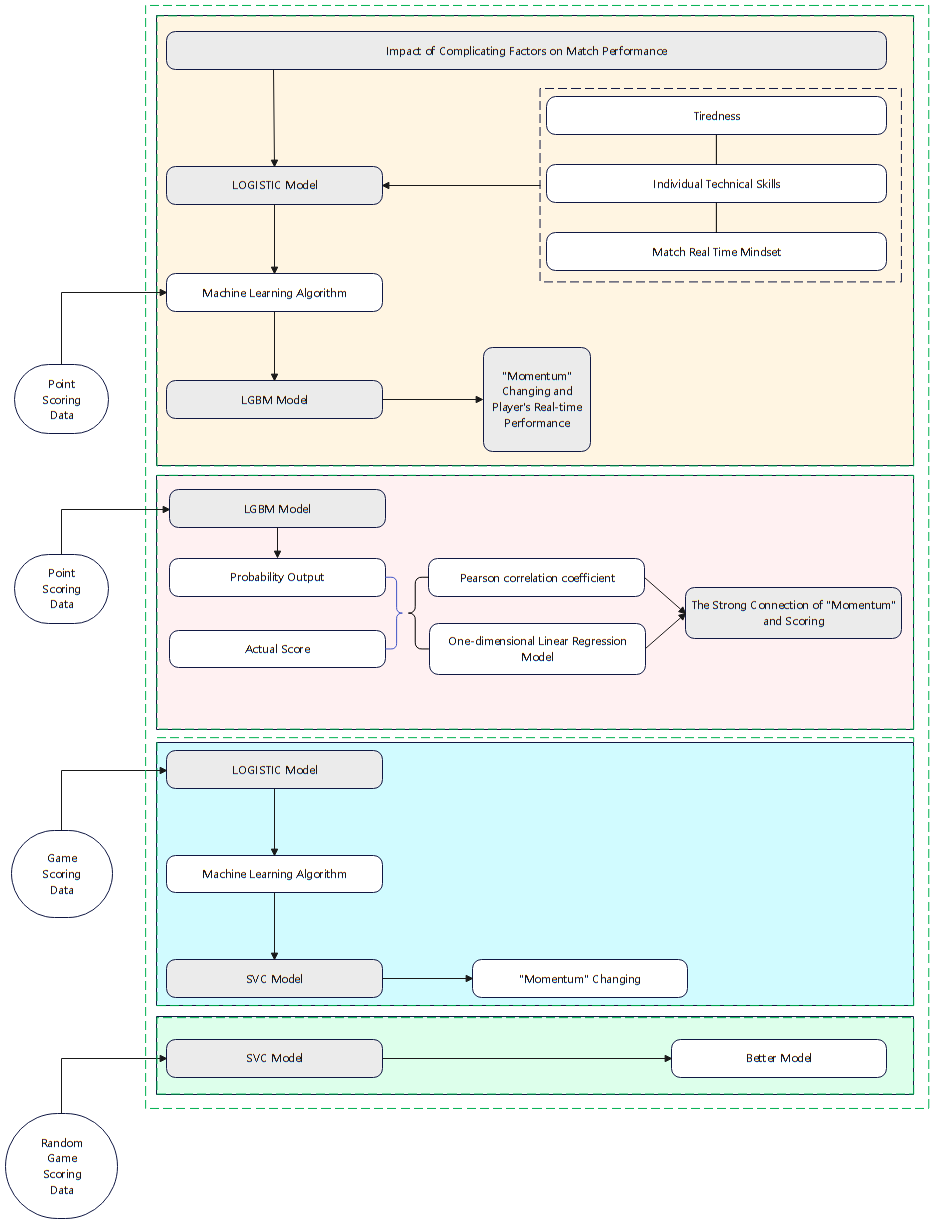
\includegraphics[width=0.5\textwidth]{floatChart.png}
      \caption{Float Chart}
\end{figure}
\section{Problem Analysis}
In the first study, multiple key factors affecting the scoring abilities of tennis players were comprehensively considered. This included not only whether they were serving but also factors like their level of fatigue, technical skills, and psychological state during the match. A comprehensive evaluation system was designed to deeply analyze these variables, such as individual technical levels, degrees of fatigue, and real-time mental states during matches. By employing statistical Logistic regression, the proposed system of indicators was tested for its correlation with players' scoring, and its effectiveness was validated on a dataset of tennis matches. Machine learning techniques, including LGBM, XGBOOST, support vector machines, perceptron networks, and logistic regression, were applied along with five-fold cross-validation and multi-dimensional performance metrics. The gradient boosting algorithm LGBM was ultimately chosen to dynamically assess players' real-time performance, or what is referred to as match "momentum."

The second study focused on exploring whether the "momentum" effect during matches has statistical significance, that is, whether the fluctuations in players' scoring during matches are non-random. The optimized machine learning model developed in the first study was applied to a test dataset, with predicted scoring probabilities compared to actual scoring records of athletes, and validated through Pearson correlation analysis. Subsequently, a univariate linear regression model was established, using predicted "momentum" as the independent variable and players' scoring as the dependent variable, to quantify the impact of "momentum" on scoring.

The third study addressed the challenges of model construction, as the model from the first study primarily focused on predicting the scoring probability of each serve and shot, rather than volatility prediction. To bridge this gap, the predictive focus was adjusted from individual shots to the outcome of entire games, analyzing fluctuations in players' performances across individual sets and the entire match. By aggregating features, a predictive model was built using statistical Logistic regression, with the support vector machine chosen as the final model. Model performance was evaluated using LGBM, XGBOOST, recall, precision, F1 score, AUC, and ROC curves. The information gain method was employed to determine the importance of various variables in the indicator system, leading to recommendations for athletes' future performance in matches.

In the final study, by selecting four matches as a validation set and using other match data as a training set, the visualization method of the ROC-AUC curve showcased the model's performance differences across various matches. Considering the uncertainty of the "volatility" indicator, machine learning evaluation standards were used for performance evaluation. In tests across these four matches, the constructed model demonstrated significant performance differences. Given this, expandable research directions were proposed, emphasizing the importance of individual athlete abilities and proving the applicability and strong generalizability of the proposed indicator system in other competitions


\section{Model Assumption}
\begin{enumerate}
\item The server has a greater advantage over the receiver.This assumption posits that the player initiating the serve in a game is more likely to gain an upper hand.
\item Players are affected by the "momentum" of the match.It's assumed that the success or failure of players during a match influences their future performance, suggesting that momentum plays a critical role in the outcome of the game.
\item A player's technical skill has a significant and direct impact on their scoring performance.This assumption highlights the importance of individual skills and how they translate into points on the board.
\item Fatigue affects players during the match, impacting their performance in the later stages.This suggests that as the match progresses, players' energy levels and their ability to maintain peak performance diminish.
\item The psychological state of players, including their ability to handle mistakes and respond to critical moments, significantly influences the match.This assumption underscores the importance of mental toughness and psychological preparedness in determining a player's success in competition.
\end{enumerate}
\section{Symbol Description}
\begin{table}[H]
\centering
\begin{tabular}{|>{\centering\arraybackslash}m{2.5cm}|p{0.6\textwidth}|}
\hline
\textbf{Symbol} & \textbf{Description} \\ \hline
$S1$ & The number of game winning in the current set \\ \hline
$S2$ & The leading scores in the current game \\ \hline
$S3$ & Whether it is the server \\ \hline
$S4$ & Whether score in the last point \\ \hline
$S5$ & The score lead progress of this match\\ \hline
$S6$ & Whether the serve is scored (no contact) \\ \hline
$S7$ & Whether to score on a return kick (no touch). \\ \hline
$S8$ & No touch score on the backhand \\ \hline
$S9$ & Is there a double fault in this game? \\ \hline
$S10$ & Whether there were unforced errors in this game. \\ \hline
$S11$ & The ratio of the number of net to the number of times score by net \\ \hline
$S12$ & The ratio of the chance of scoring when the opponent serves to the number of points actually scored. \\ \hline
$S13$ & Total mileage in this match \\ \hline
$S14$ & The total mileage in the last three points \\ \hline
$S15$ & Mileage chart from last point \\ \hline
$S16$ & Serve real-time pace \\ \hline
\end{tabular}
\caption{Symbol Description}
\end{table}
\section{Model Construction and Analysis}
\subsection{Task1: Model Construction}
\subsubsection{Data Preprocessing}
In the initial phase of data preprocessing, the dataset is imported from a .csv file, and the Pandas library is employed to structure the data into a DataFrame. Subsequent to this, the dropna function is applied to eliminate records with missing values. Following the initial data preparation, the script undertakes a comprehensive feature engineering process, introducing novel features pertinent to the distinct characteristics of tennis matches.

In the subsequent phase, the dataset is readied for modeling through a meticulous iteration over each data point. This involves the extraction of features and the assignment of labels contingent upon the outcome of each point, specifically focusing on point victories. To enhance the robustness and suitability of the data for subsequent machine learning applications, the features undergo scaling. The MinMaxScaler from the scikit-learn library is employed for this purpose, ensuring that all variables are standardized within the [0, 1] range. This standardization is imperative to mitigate the undue influence of certain features during the modeling process, arising from variations in scale.

The finalization of the preprocessing sequence involves the preservation of the processed and standardized dataset in an Excel file. These methodical steps collectively address challenges associated with missing values, outliers, and standardization, culminating in the generation of a refined dataset poised for efficacious utilization in machine learning endeavors.
\subsubsection{Model Analysis}
The analysis of player performance in tennis is a multifaceted task that requires a comprehensive approach, blending traditional statistical methods with advanced machine learning techniques. In this section, we delve into the intricacies of our model, examining the preprocessing steps, model training, evaluation metrics, and the overall performance against various benchmarks.

Initially, we employed logistic regression to assess the statistical significance of the relationship between our established indicator system and the corresponding labels. Leveraging a tennis match dataset, we computed these indicators and labels indicating player scoring. This step not only aids in comprehending how various factors impact a player's score but also lays a crucial groundwork for feature selection in the modeling phase.

Subsequent to this, we utilized a range of machine learning algorithms, including LGBM, XGBoost, Support Vector Machines, Perceptron Networks, and Logistic Regression. We compared their effectiveness using metrics like accuracy, recall, precision, F1-score, AUC, and ROC curves. This step not only robustly supports our final choice of the LGBM algorithm for modeling but also ensures the model's capacity for generalization.

In the concluding phase, we opted for the LGBM algorithm for modeling. This algorithm not only dynamically evaluates a player's performance but also captures shifts in "momentum" during a match. This dynamic assessment model facilitates more accurate predictions of a player's performance, enhancing the precision of predicting match outcomes. Through this research, we have taken a noteworthy stride in comprehending and appraising player tactics and scoring, establishing a strong basis for more in-depth analysis and prediction.

Concerning the creation of the indicator system, we analyzed potential factors influencing a tennis player's scoring. The system was formulated based on elements like player fatigue, real-time and historical scoring situations, and the player's psychological state. This thorough analysis contributes to a nuanced understanding of player performance, paving the way for further exploration and prediction.

\subsubsection{Index Creation}
we analyze the factors that might correlate with the player's score. According to the player's fatigue and mental state etc., make an index system as follows.

\begin{table}[H]
      \centering
      \begin{tabular}{|>{\centering\arraybackslash}m{2.5cm}|p{0.6\textwidth}|}
      \hline
      \textbf{Categery} & \textbf{Index} \\ \hline
      Fatigue &  Total mileage in this match\\ \hline
      Fatigue &  The total mileage in the last three points \\ \hline
      Fatigue &  Whether score in the last point \\ \hline
      State & Whether there is a double fault \\ \hline
      State & Whether there were unforced errors in this game.\\ \hline
      State & Serve real-time pace  \\ \hline
      State & Whether it is an interactive item for the server's serving pace\\ \hline
      State &  The ratio of the number of net to the number of times score by net\\ \hline
      State & The ratio of the chance of scoring when the opponent serves to the number of points actually scored.\\ \hline
      Ability& Whether the serve is scored (no contact) \\ \hline
      Ability& Whether to score on a return kick (no touch). \\ \hline
      Ability& No touch score on the backhand \\ \hline
      Ability& The score lead progress of this match\\ \hline
      Ability& The leading scores in the current game \\ \hline
      Ability& The number of game winning in the current set \\ \hline
      Ability& Whether score in the last point \\ \hline
      Situations& Whether it is the server \\ \hline
      \end{tabular}
      \caption{Symbol Description}
\end{table}
\subsubsection{Statistical Logistic Regression Analysis Based on Indicator System}
This study employs a comprehensive indicator system to assess the impact of various factors on the real-time scoring of players in sports matches.
The indicator system allows for the calculation of scores for each point in every set of every match played by a participant, with corresponding assessments
of the player's current performance indicators. To validate the significance of the indicators within this system concerning point scoring, a statistical regression analysis is conducted.
Given the binary nature of point scoring outcomes, a binary logistic regression model is selected, and the analysis is executed using SPSS software[2].
\begin{figure}[H]
      \centering
      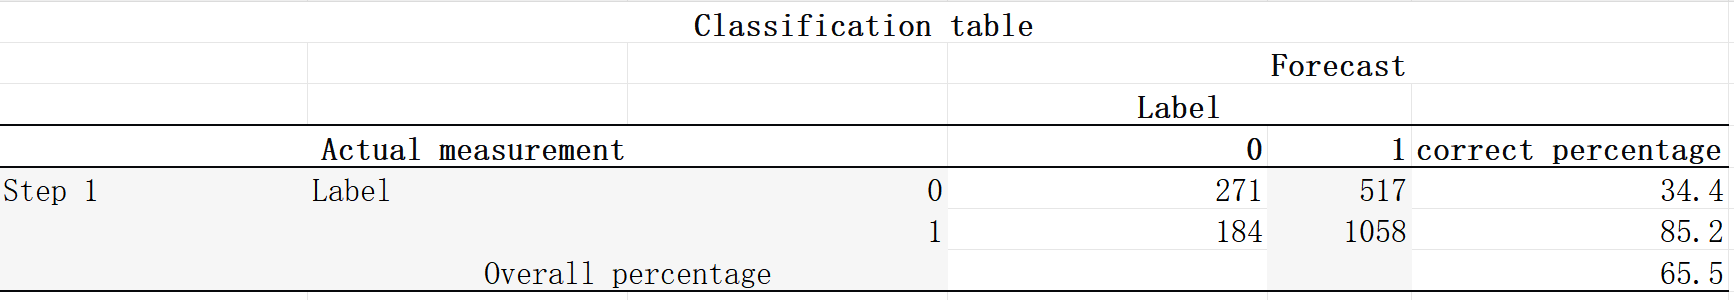
\includegraphics[width=0.7\textwidth]{logistic_classfication_1.png}
      \caption{logistic regression performance}
\end{figure}
The logistic regression analysis in SPSS yielded an overall accuracy of 65.5\%. The model exhibited a classification accuracy of 34.4\%
for instances where players genuinely did not score, while achieving a significantly higher accuracy of 85.2\% for instances where players did score.
This suggests a preference of the model to classify samples into situations where players actually scored (label 1).

However, it is crucial to note that this logistic regression analysis provides a prospective examination. Its purpose is to investigate
whether the constructed indicators significantly influence the actual scoring situation of players. The results of the logistic regression analysis are presented in the following table.

\begin{figure}[H]
      \centering
      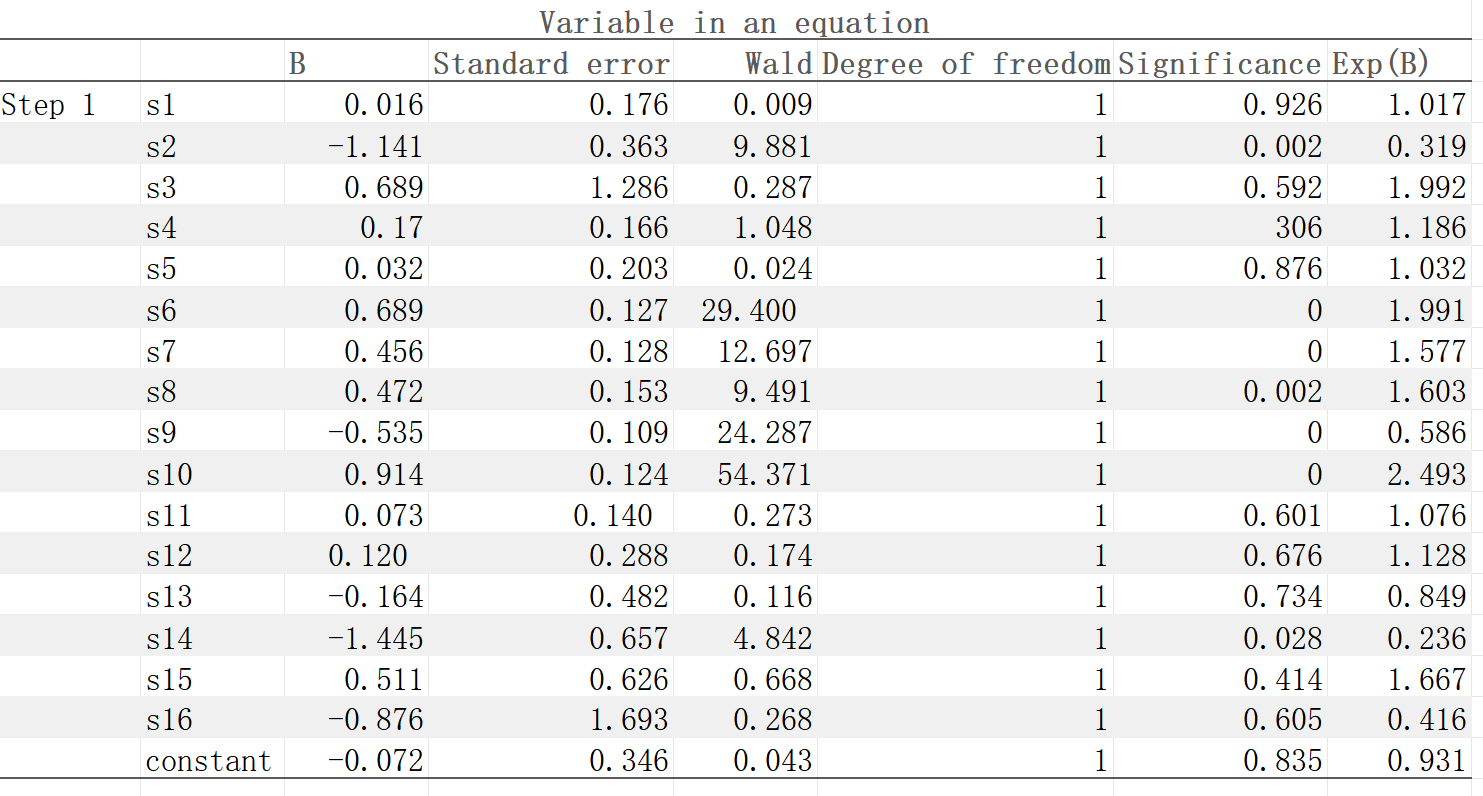
\includegraphics[width=0.7\textwidth]{variable_eq1.png}
      \caption{Logistic regression results}
\end{figure}
As the figure table shows, the p-values for the majority of the independent variables are less than 0.05, indicating a significant influence of these variables on the dependent variable. Consequently, in this indicator system,
variables such as s2, s6, s7, s8, s10, and s14 have been identified as significantly affecting a player's real-time scoring situation.
This suggests that both a player's individual abilities and factors like fatigue or psychological state can exert a significant impact on their real-time scoring performance.

\subsubsection{Evaluation of Machine Learning Models Based on an Indicator System}
The model construction phase involves the selection of high-performing ensemble tree models, specifically LightGBM (LGBM) and XGBoost, alongside classical machine learning algorithms,
namely Support Vector Machine (SVM), Perceptron Neural Network, and Logistic Regression, serving as comparative benchmarks. The models are validated using k-fold cross-validation,
and performance metrics such as accuracy, precision, recall, F1 score, and AUC-ROC curve are derived from confusion matrices[1].

The confusion matrix-based results are presented in the table below, while the training and testing outcomes based on AUC-ROC curves are illustrated in the figures[3].
\begin{figure}[H]
      \centering
      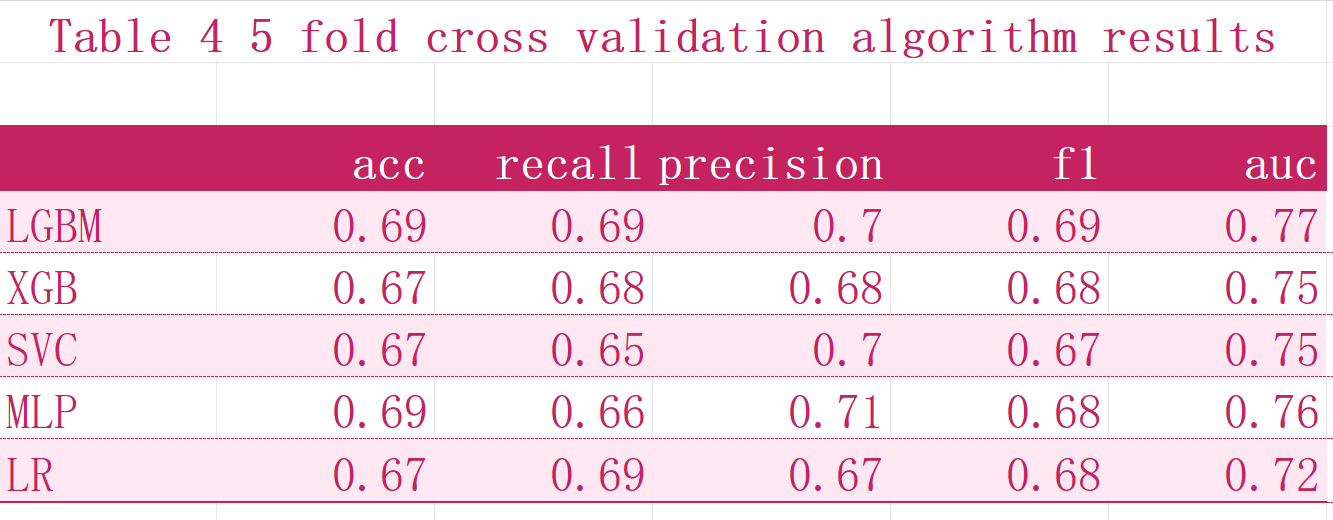
\includegraphics[width=0.7\textwidth]{crossValidation.png}
      \caption{Cross Valadation}
\end{figure}

Among the models, LGBM exhibits superior performance with accuracy, precision, recall, F1 score, and AUC values of 0.69, 0.69, 0.77, 0.69, and AUC\_L respectively. Neural Network follows closely, demonstrating minimal discrepancies in metrics (0.69, 0.66, 0.71, 0.68, AUC\_NN), indicating a lack of pronounced bias in positive or negative sample discrimination. Consequently, the effectiveness of LGBM is affirmed.
\begin{figure}[H]
      \centering
      \begin{subfigure}{0.48\textwidth} % Adjust the width as needed
          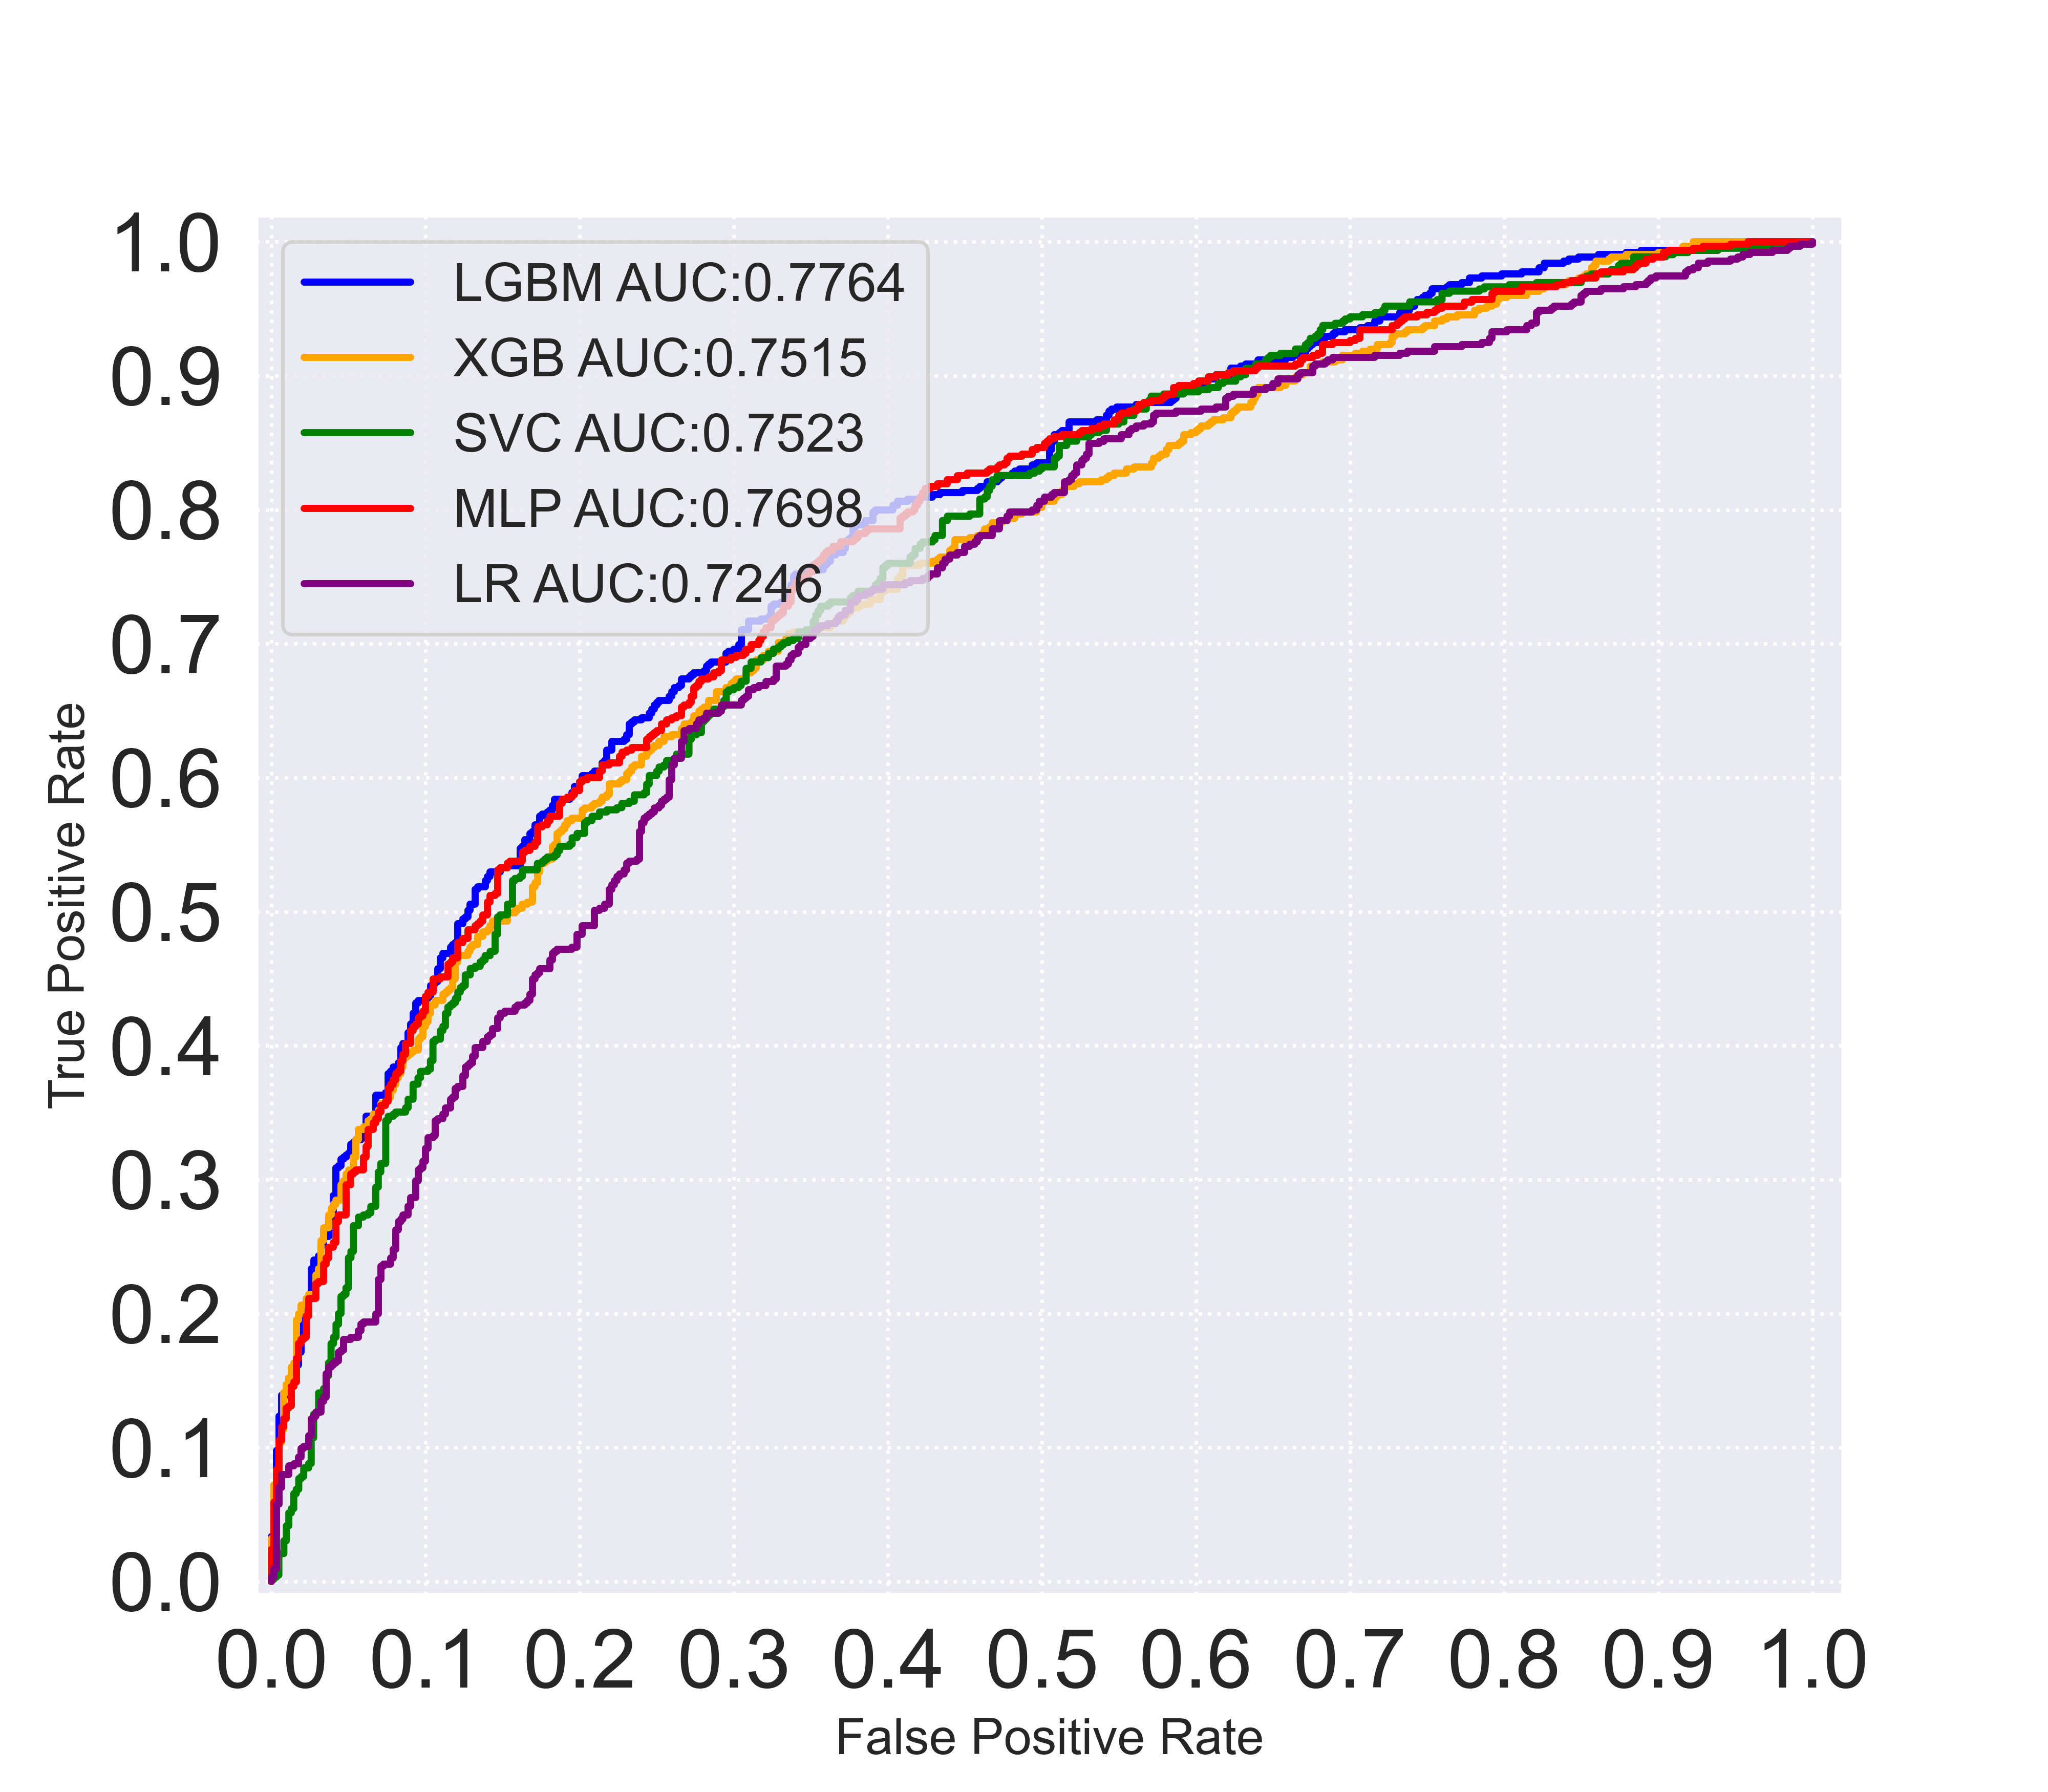
\includegraphics[width=\linewidth]{roc_auc(test(before_sampling)).png} % Replace 'figure1' with the filename of your first figure
          \caption{Test}
          \label{fig:roctest}
      \end{subfigure}
      \hfill % Add horizontal space between the subfigures
      \begin{subfigure}{0.48\textwidth} % Adjust the width as needed
          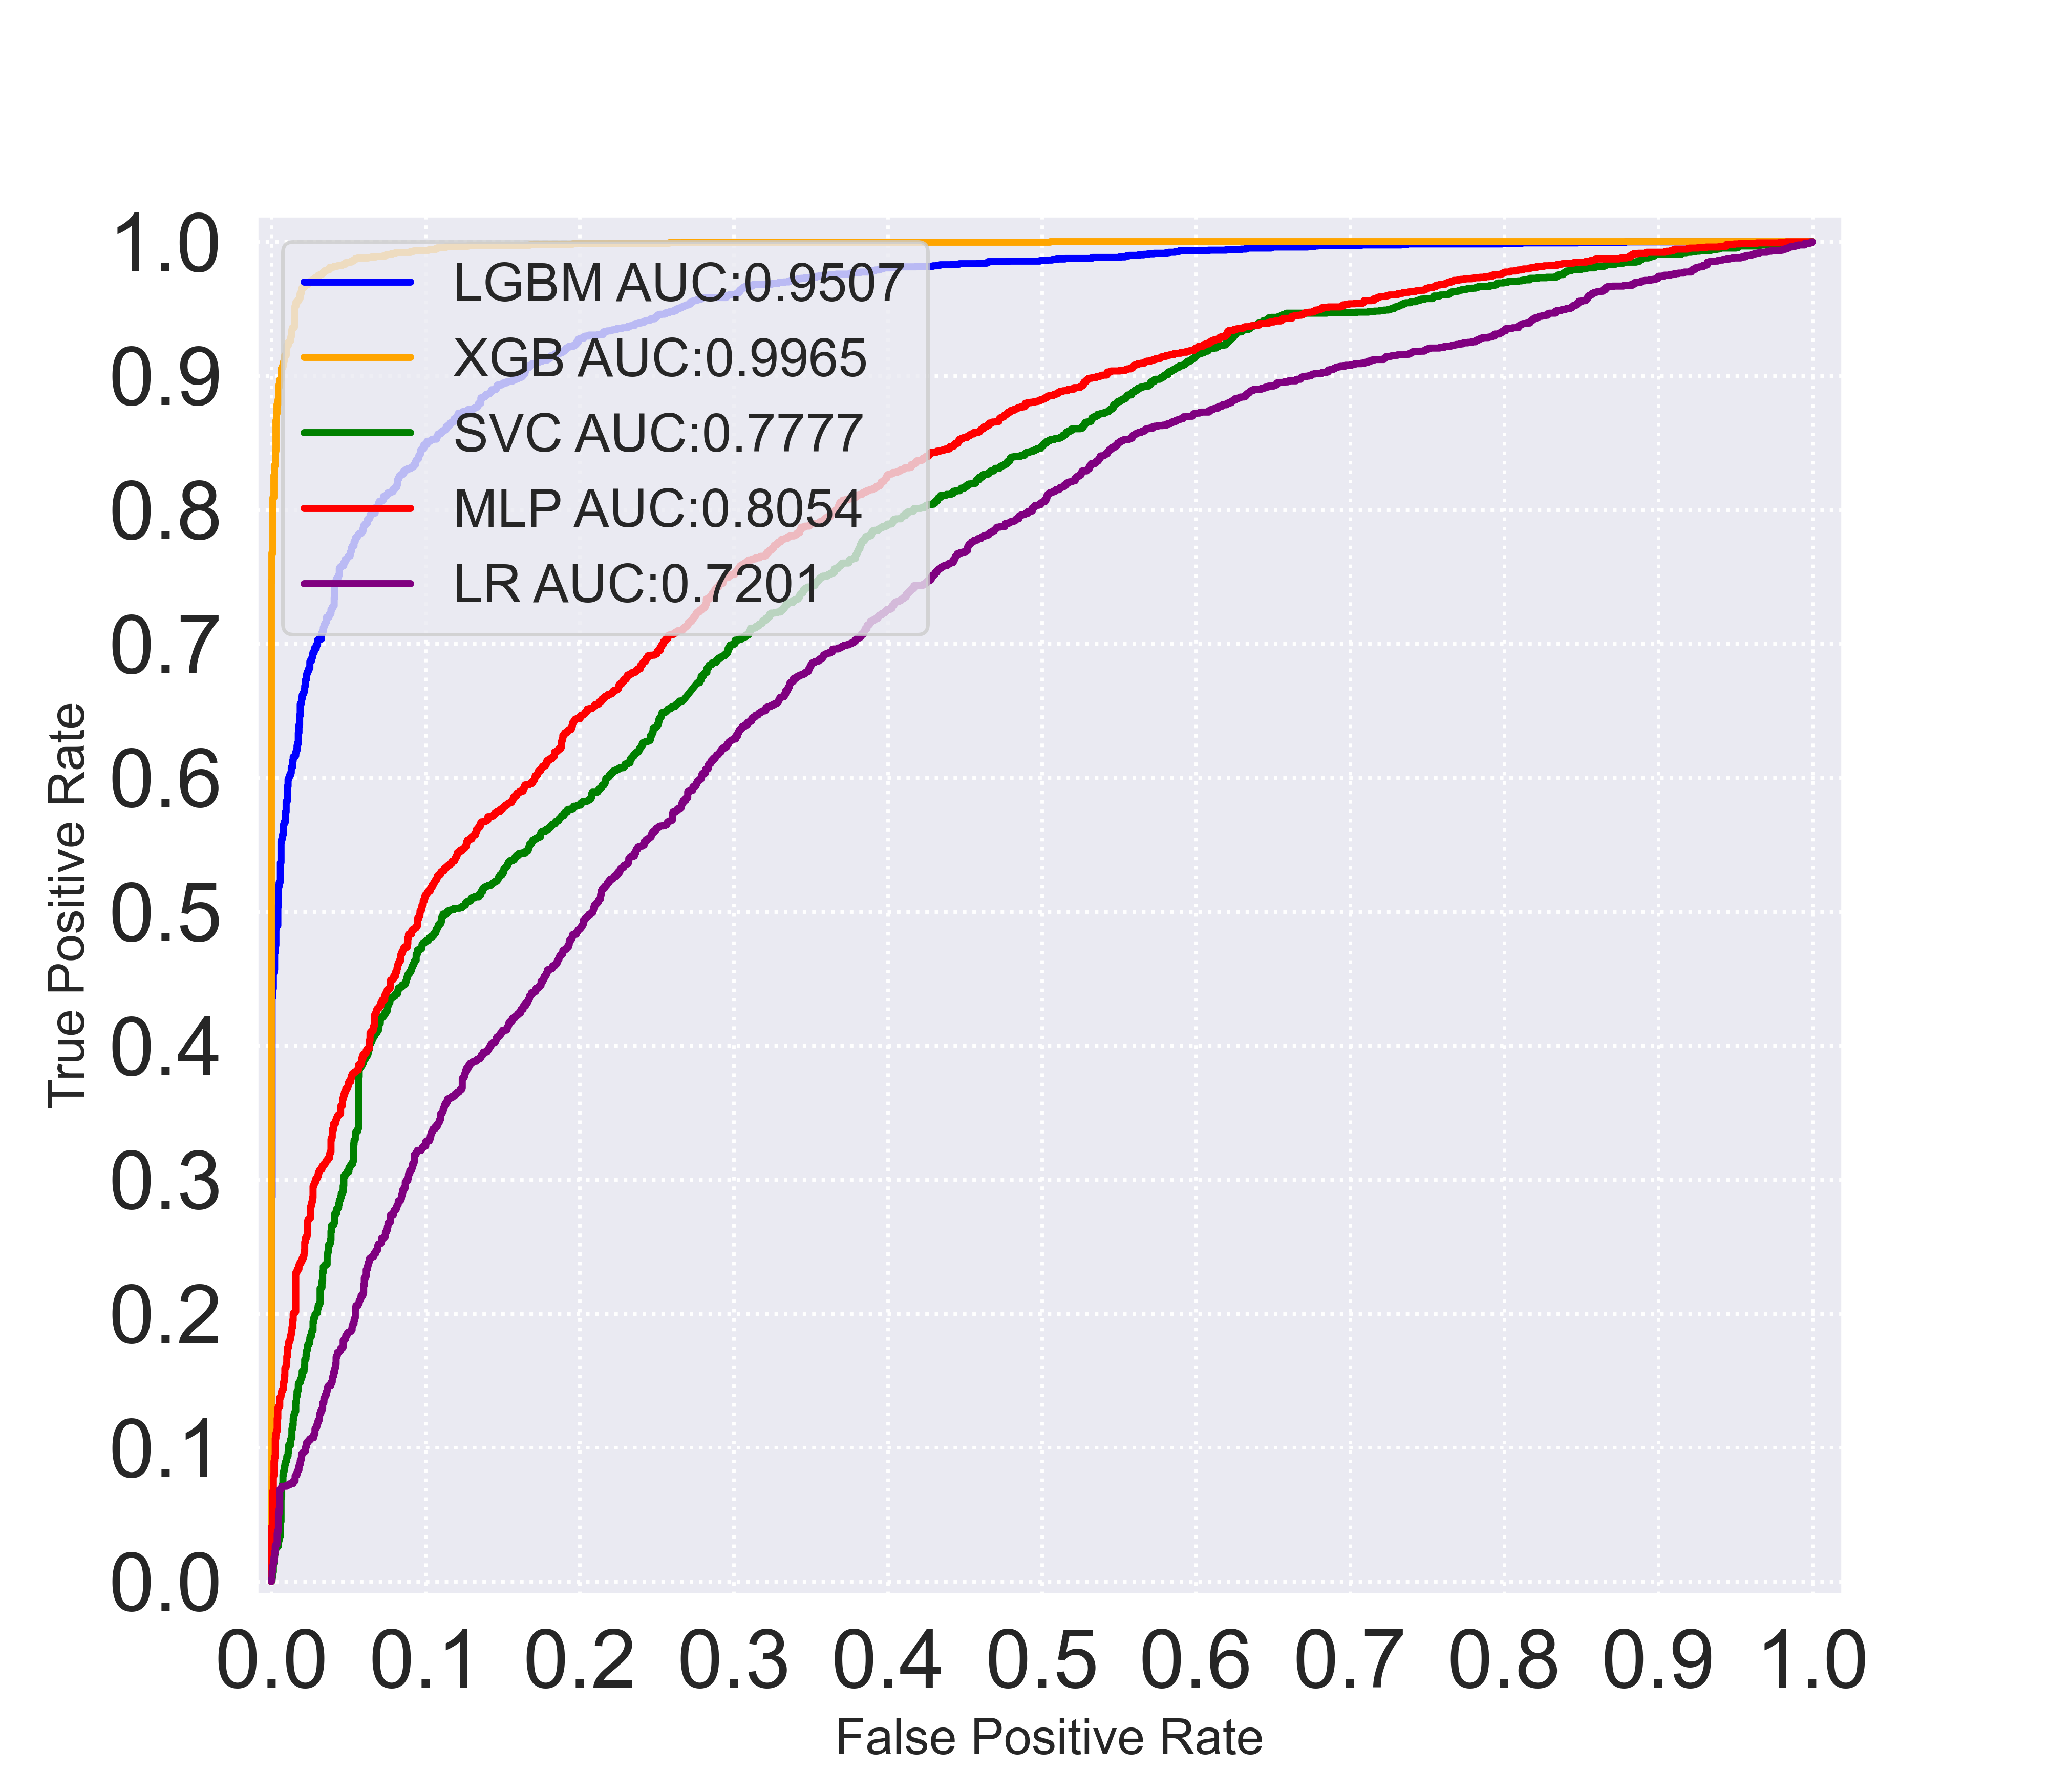
\includegraphics[width=\linewidth]{roc_auc(train(before_sampling)).png} % Replace 'figure2' with the filename of your second figure
          \caption{Train}
          \label{fig:roctrain}
      \end{subfigure}
      \caption{Task 1 Overall performance of the model}
      \label{fig:overall}
\end{figure}

The ROC curves illustrate variations in precision and recall metrics at different threshold settings. Through ROC analysis, it further validates LGBM as the most effective algorithm.

Building upon these findings, a new training model is established utilizing the top-performing LGBM model. Real-time performance visualization is conducted on the classic match between 20-year-old rising Spanish star Carlos Alcaraz and 36-year-old Novak Djokovic in the 2023 Wimbledon Men's Singles Final. The result is shown as follows.
\begin{figure}[H]
      \centering
      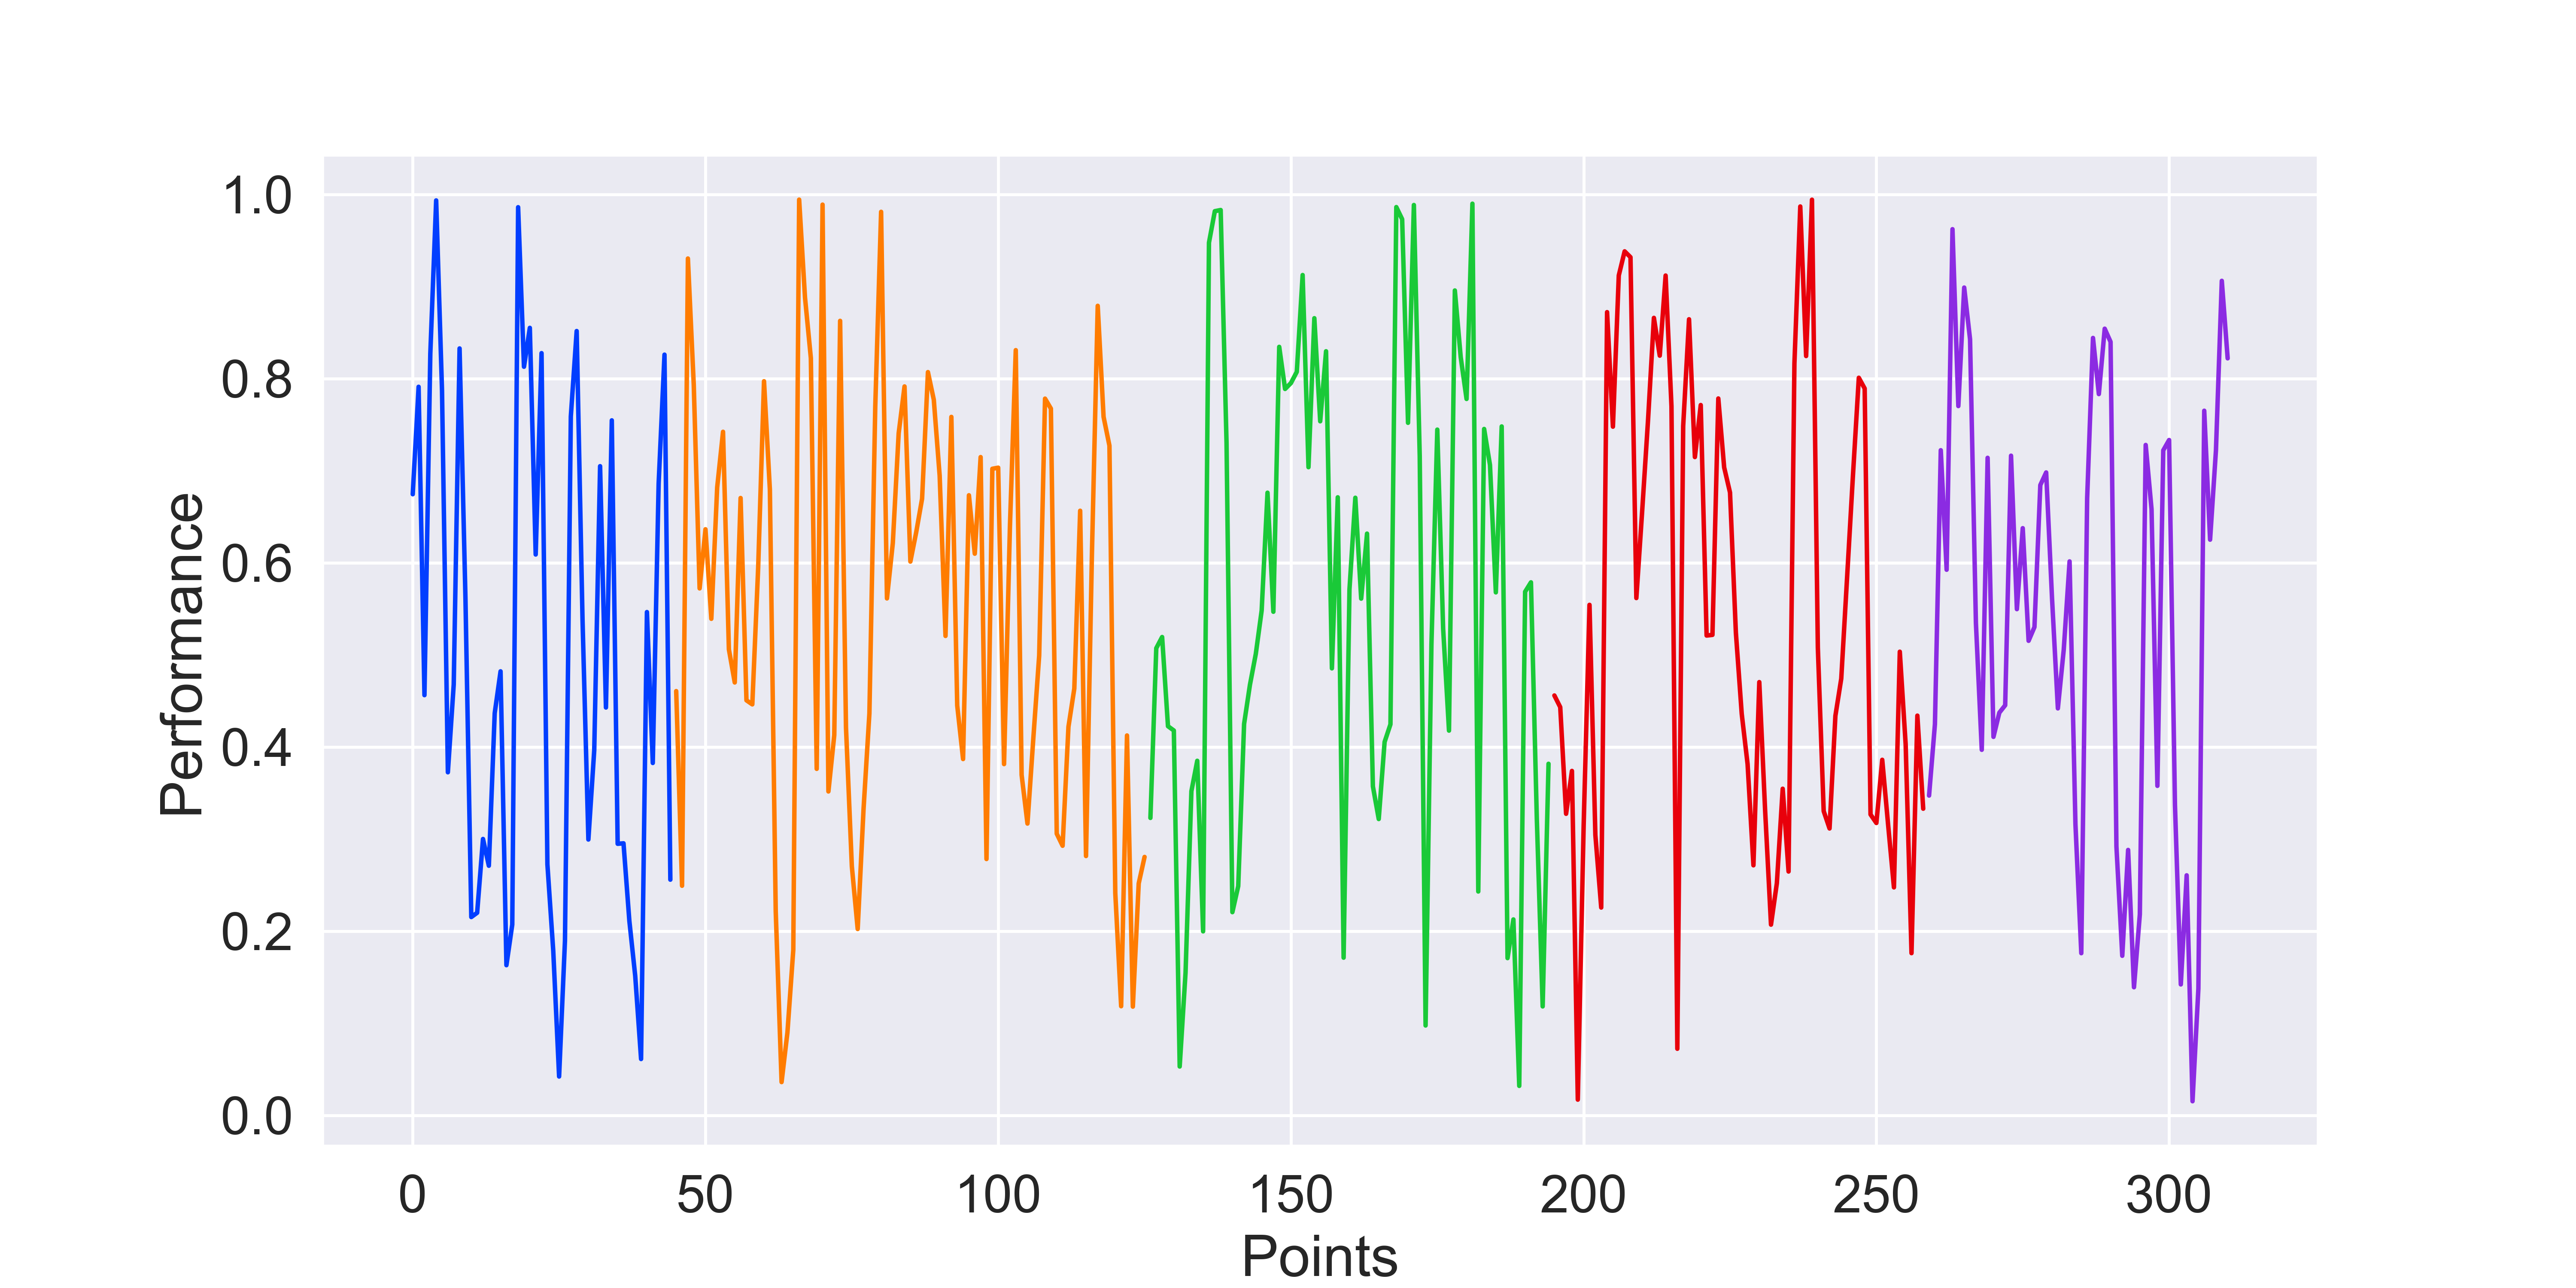
\includegraphics[width=0.7\textwidth]{classic_duel_trend.png}
      \caption{Classic duel}
\end{figure}

In fact, the predictive accuracy for scoring points has no upper limit, which aligns with our intuition. The complexity of factors influencing whether a player can score is highly intricate.
Without considering these complex elements, the noise in a player's performance becomes significantly pronounced. As a result, the model can accurately discern the real scoring situations of only approximately 70\%
of the players. We observe that in this classic match, the server and scorer precisely align with the actual scoring situations of the players. When Carlos Alcaraz secures victory, the momentum is high, and it is relatively low when facing defeat.
This indicates that the model remains effective, as it reflects the consistency between the classic battle outcomes and the real-time scoring situations of the players.
\subsection{Task2}
\subsubsection{Task2: Model Analysis}
In the second phase of our research, we are dedicated to gaining a deeper understanding of the practical role of "momentum" in sports competitions. The aim is to unveil whether the fluctuations and successes exhibited by players during a match demonstrate a non-random trend.
To achieve this objective, I initially applied the optimal machine learning model established in Task one to the test set, generating probability outputs for player scoring. Through Pearson correlation tests between these outputs and the actual player scoring situations,
we attempt to identify the degree of association between the output probabilities and the real scoring outcomes.

Furthermore, we employ a univariate linear regression model, where the predicted "momentum" serves as the independent variable and the player's actual scoring as the dependent variable. Through this modeling process, we not only track the impact of momentum on real-time scoring
but also endeavor to uncover the interpretable components behind the "momentum." This in-depth analytical process aims to reveal the exact mechanisms through which "momentum" influences player scoring, providing a more comprehensive understanding of the dynamic characteristics of player performance.

Within this research framework, we anticipate concluding that "momentum" is not merely a simple random phenomenon but indeed exerts a noticeable and meaningful impact on player scoring. Through these efforts, we aim to offer a more detailed and profound insight into the practical significance
of momentum in sports competitions, providing specific recommendations and guidance for player performance during matches.
\subsubsection{Pearson Correlation Test}
\textbf{Principles of Pearson Correlation Test}\\

The Pearson correlation coefficient is a statistical measure used to assess the linear relationship between two variables, with values ranging from -1 to 1. Specifically:

\begin{itemize}
  \item A value of 1 indicates a perfect positive correlation: when one variable increases, the other variable increases correspondingly.
  \item A value of -1 indicates a perfect negative correlation: when one variable increases, the other variable decreases.
  \item A value of 0 suggests no linear relationship.
\end{itemize}

The calculation formula for the Pearson correlation coefficient (often denoted by the symbol \(r\)) is as follows:

\[ r = \frac{\sum{(x_i - \bar{x})(y_i - \bar{y})}}{\sqrt{\sum{(x_i - \bar{x})^2} \cdot \sum{(y_i - \bar{y})^2}}} \]
\\
Here, \( x_i \) and \( y_i \) are the corresponding data points, \( \bar{x} \) and \( \bar{y} \) are the respective means of the variables. The numerator represents the sum of the product of the deviations of each data point from their respective means, while the denominator signifies the square root of the product of the sums of squared deviations for both variables.

A computed \( r \) value closer to 1 or -1 indicates a stronger linear relationship between the two variables. Conversely, an \( r \) value close to 0 suggests a lack of linear relationship between the variables.
\\
\textbf{Pearson Correlation Test Results}\\

As the goal is to demonstrate whether the momentum output by the model can influence the players' actual performance, it is necessary to establish the significance of their correlation.
\begin{table}[H]
      \centering
      \begin{tabular}{|c|c|}
      \hline
      \textbf{Correlation coefficient} & \textbf{P Value} \\ \hline
      0.482 &  0.000\\ \hline
      \end{tabular}
      \caption{Pearson result}
\end{table}
It is observed that the p-value is less than 0.05, indicating a significant correlation between momentum and player performance. Furthermore, this relationship is characterized as a positive correlation, signifying that a larger momentum corresponds to better player performance and an increased likelihood of scoring.

\subsubsection{Univariate Linear Regression Model}
Similarly, we use linear regression to analyze whether momentum can significantly affect player scores. The result is as shown below:
\begin{figure}[H]
      \centering
      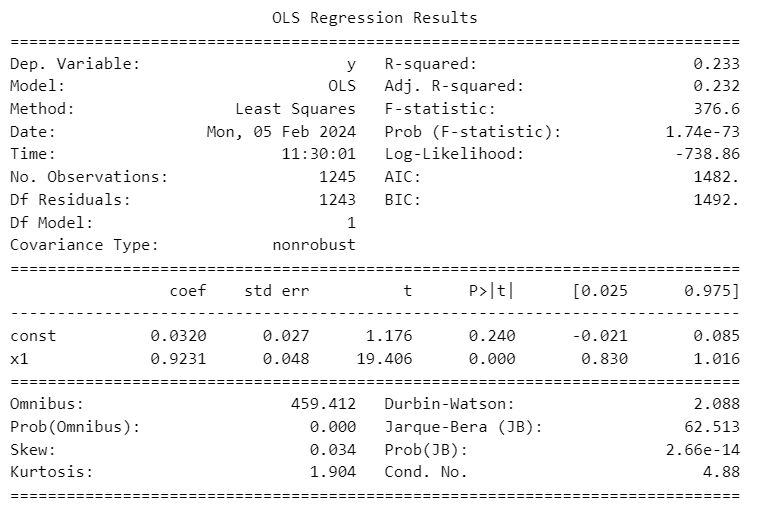
\includegraphics[width=0.7\textwidth]{Univariate_linear_regression.png}
      \caption{Univariate regression}
\end{figure}
It can be seen that the p-value of momentum is also less than 0.05, and its weight is 0.9231. The impact of momentum x1 on the results is significant, and it can explain 0.233 of the results.

\subsection{Task3: Reflecting player performance fluctuations throughout the game}
In the study of Task three, we deeply analyzed the limitations of the established model. This model mainly focuses on predicting the score of each player's serve and stroke, and is therefore limited to having high randomness. To overcome one of the limitations, we adopted a more nuanced approach designed to more accurately reflect ,player performance fluctuations throughout the game.

First, we upgraded the model in Task 1 to aggregate features and calculate the player's single game win. This new prediction goal provides us with more specific and accurate data, allowing us to better understand Player performance in the game. Subsequently, we again used statistical LOGISTI to build a model to determine the significant impact of the proposed indicator system on predicting game results.

Comparing the results of Task 1, we found that the indicator system proposed in the text has a more significant impact on the independent variables in game prediction. In the comparative analysis of multiple machine learning algorithms, especially LGBM, XGBOOST, support vector machine, perceptron network, and logistic regression, the support vector machine performed well and became the best model we selected. In order to further strengthen the model For interpretability, we used the information gain method to calculate the importance score of the indicator system, which helps us understand the specific contribution of each indicator to the players.

In the end, we not only provided an excellent support vector machine model for modeling player performance fluctuations, but also gained a deeper understanding of the importance of the indicator system through the analysis of information gain. At the end of the study,
we provide performance recommendations for players when entering new games, aiming to help players achieve better performance in the game. These recommendations are not only based on our model results, but also incorporate the overall status of the players and specific
situations. Deep insights provide players with more comprehensive support.

\subsection{Logistic Test With Game as Granularity}
Similarly, we use statistical logistic regression for testing. The results are shown in the table
\begin{figure}[H]
      \centering
      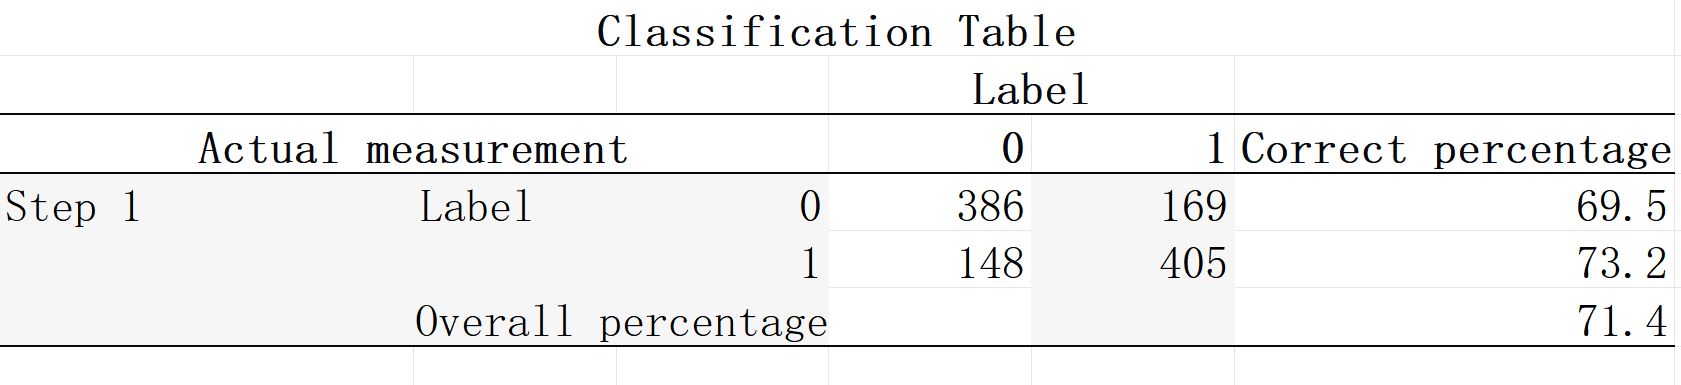
\includegraphics[width=0.7\textwidth]{logisitc_classification2.png}
      \caption{Logistic regression performance of game granularity}
\end{figure}
It can be seen that compared to point-based logistic regression, the accuracy of game-based logistic regression has a clear value-added,
from 65.5 to 71.4. At this time, the results of the model can better reflect the real fluctuation state of the players. Then, the results of the logistic
regression test are as shown in the figure
\begin{figure}[H]
      \centering
      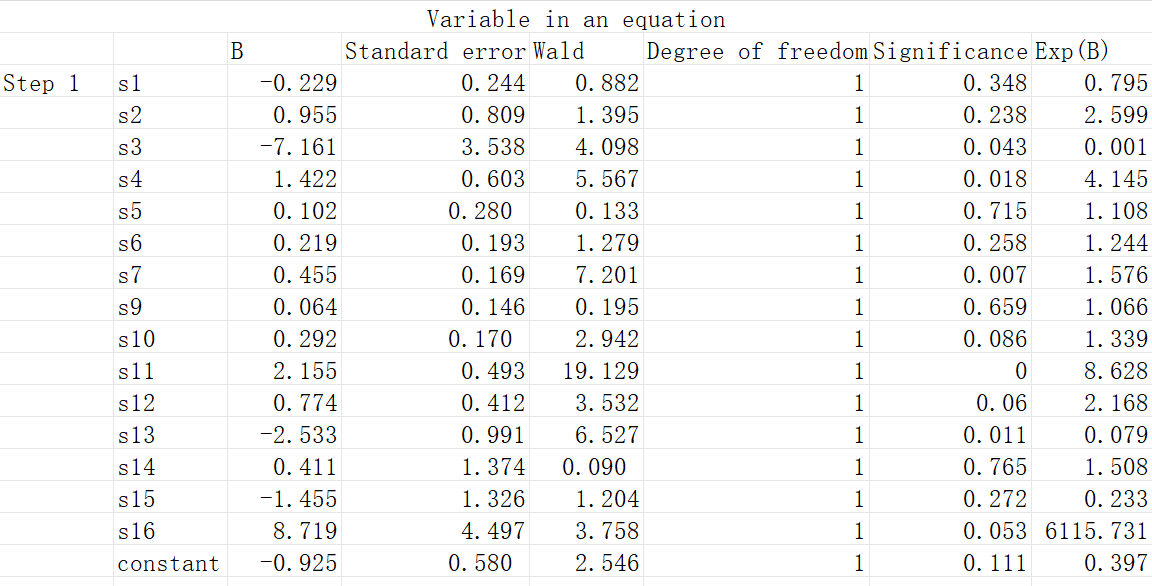
\includegraphics[width=0.7\textwidth]{logistic_eq2.png}
      \caption{Logistic regression results of game granularity}
\end{figure}
Compared with the results of Task 1, in the existing results, many variables that were originally insignificant became significant, including x3, x4, x11 and x13

\subsubsection{Evaluation of Machine Learning Models Based on an Indicator System}
In addition, as before, because the performance of binary logistic regression itself is limited, we hope to use a better model for prediction,
so we use some classic machine learning algorithms for evaluation, such as accuracy, recall, precision, f1 Evaluate with auc, and use the fold-free cross-validation method for verification. T he results are as follows:
\begin{figure}[H]
      \centering
      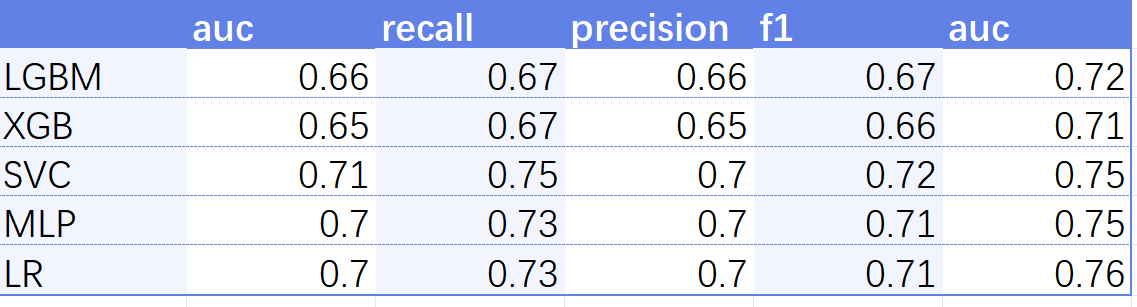
\includegraphics[width=0.7\textwidth]{crossValidation2.png}
      \caption{Cross Valadation}
\end{figure}

This time, the best performer is SVC, whose accuracy, precision, recall, f1 and auc are 0.71, 0.75, 0.7, 0.72 and 0.75 respectively,
followed by LR, which is 0.7, 0.76, 0.71 and 0.73. The recall index is the best in the entire model, indicating that the model has certain preferences[8]. On the other hand, the model
with game granularity has better performance in the classic model, but the effect of the tree model is not ideal. The reason may be because there are more floating-point data types with game granularity.

\begin{figure}[H]
      \centering
      \begin{subfigure}{0.48\textwidth} % Adjust the width as needed
          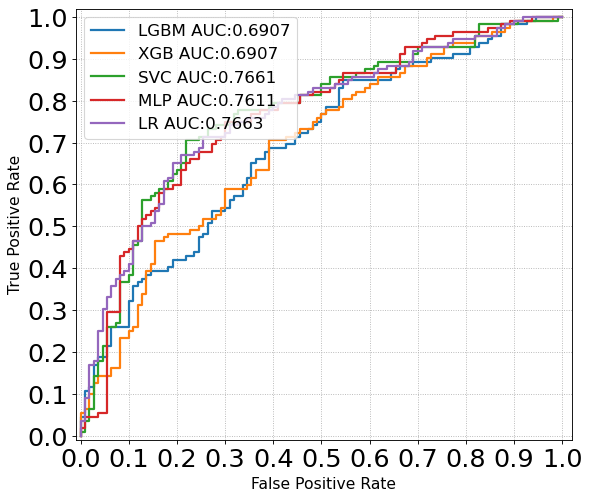
\includegraphics[width=\linewidth]{task3_auc_test.png} % Replace 'figure1' with the filename of your first figure
          \caption{Test}
          \label{fig:roctest}
      \end{subfigure}
      \hfill % Add horizontal space between the subfigures
      \begin{subfigure}{0.48\textwidth} % Adjust the width as needed
          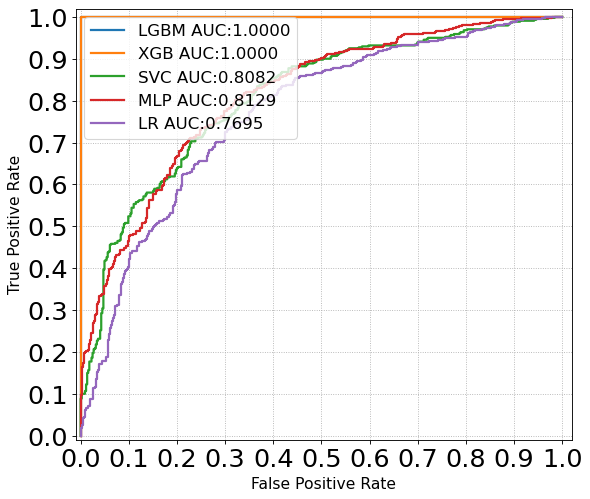
\includegraphics[width=\linewidth]{task3_auc_train.png} % Replace 'figure2' with the filename of your second figure
          \caption{Train}
          \label{fig:roctrain}
      \end{subfigure}
      \caption{Task 3 Overall performance of the model}
      \label{fig:overall}
\end{figure}
The ROC curve also shows that the vector machine has the best effect, and the training set score of the tree model is much higher than the test set, indicating that the model is overfitting[8].
\begin{figure}[H]
      \centering
      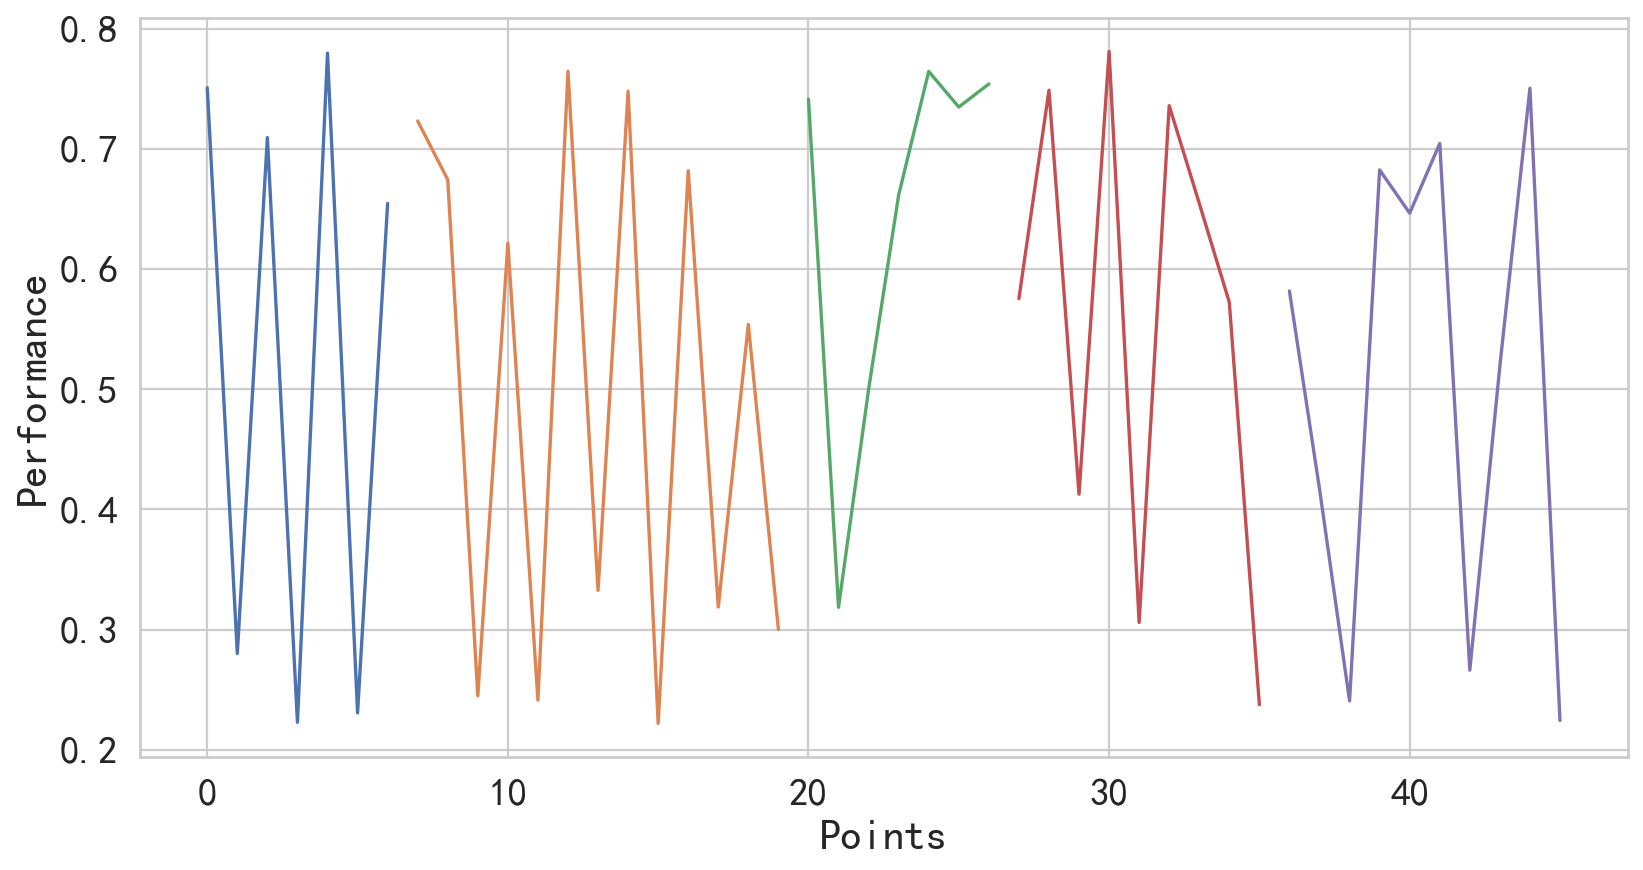
\includegraphics[width=0.7\textwidth]{duelMatch2.png}
      \caption{Duel Match Analysis 2}
\end{figure}

\subsection{Task4 and 5 Model: Systematic Case Study by Randomly Selecting 4 Games for Testing}
In the study of Tasks 4 and 5, we conducted a systematic case study by randomly selecting 4 games for testing and using the remaining data as a training set to ensure the universality and reliability
of our proposed model. sex. Through visualization with roc-auc, we clearly presented the significant differences of the model between competitions, thus verifying the robustness of the model in different competition scenarios.

Faced with the high ambiguity of the "fluctuation" indicator, we insist on using machine learning indicators for evaluation to ensure accurate measurement of model performance. Across four games, we find that the proposed model exhibits significant
performance differences, which further validates the reliability of our model.

As for the explanation of performance differences, we propose a direction worthy of further research, that is, the extremely critical role that players' personal abilities may play in this process. This insight provides implications for future research directions,
which may include further analysis of individual ability indicators and model adjustments to better capture individual differences among players in competition.

In addition, we emphasized the generalization degree of the indicator system proposed in this article. Through its application in other competition scenarios, we proved that this indicator system has good generalization. Not only can it be used in different competitions,
but it can also maintain effective predictions of the performance of flag team players. This conclusion provides a solid theoretical basis for extending the model to a broader competition context. It also provides a feasible reference for similar research in different fields in the future. Specifically,
we randomly selected 4 games, used the four games as the test set, and the remaining data as the training set. , Since the "fluctuation" indicator is fuzzy and difficult to quantify, we still use machine learning indicators for evaluation. Specifically, we visualize the auc-roc used in the four games, and then draw the specific fluctuations.

\subsection{Evaluation of Player Fluctuation Prediction Effect}
We have selected four Wimbledon men's singles matches in 2023, namely 2023-wwimbledon-1305, 2023-wwimbledon-1314, 2023-wwimbledon-1602, 2023-wwimbledon-1302. Use the model trained in Task 3 to visualize fluctuations and ROC curves. Fluctuation visualization can see the specific player fluctuations, and the ROC curve can see the prediction performance for the game. The results are as shown in the figure
\begin{figure}[H]
      \centering
      \includegraphics[width=0.55\textwidth]{fluctuation.png}
      \caption{Fluctuation}
\end{figure}
\begin{figure}[H]
      \centering
      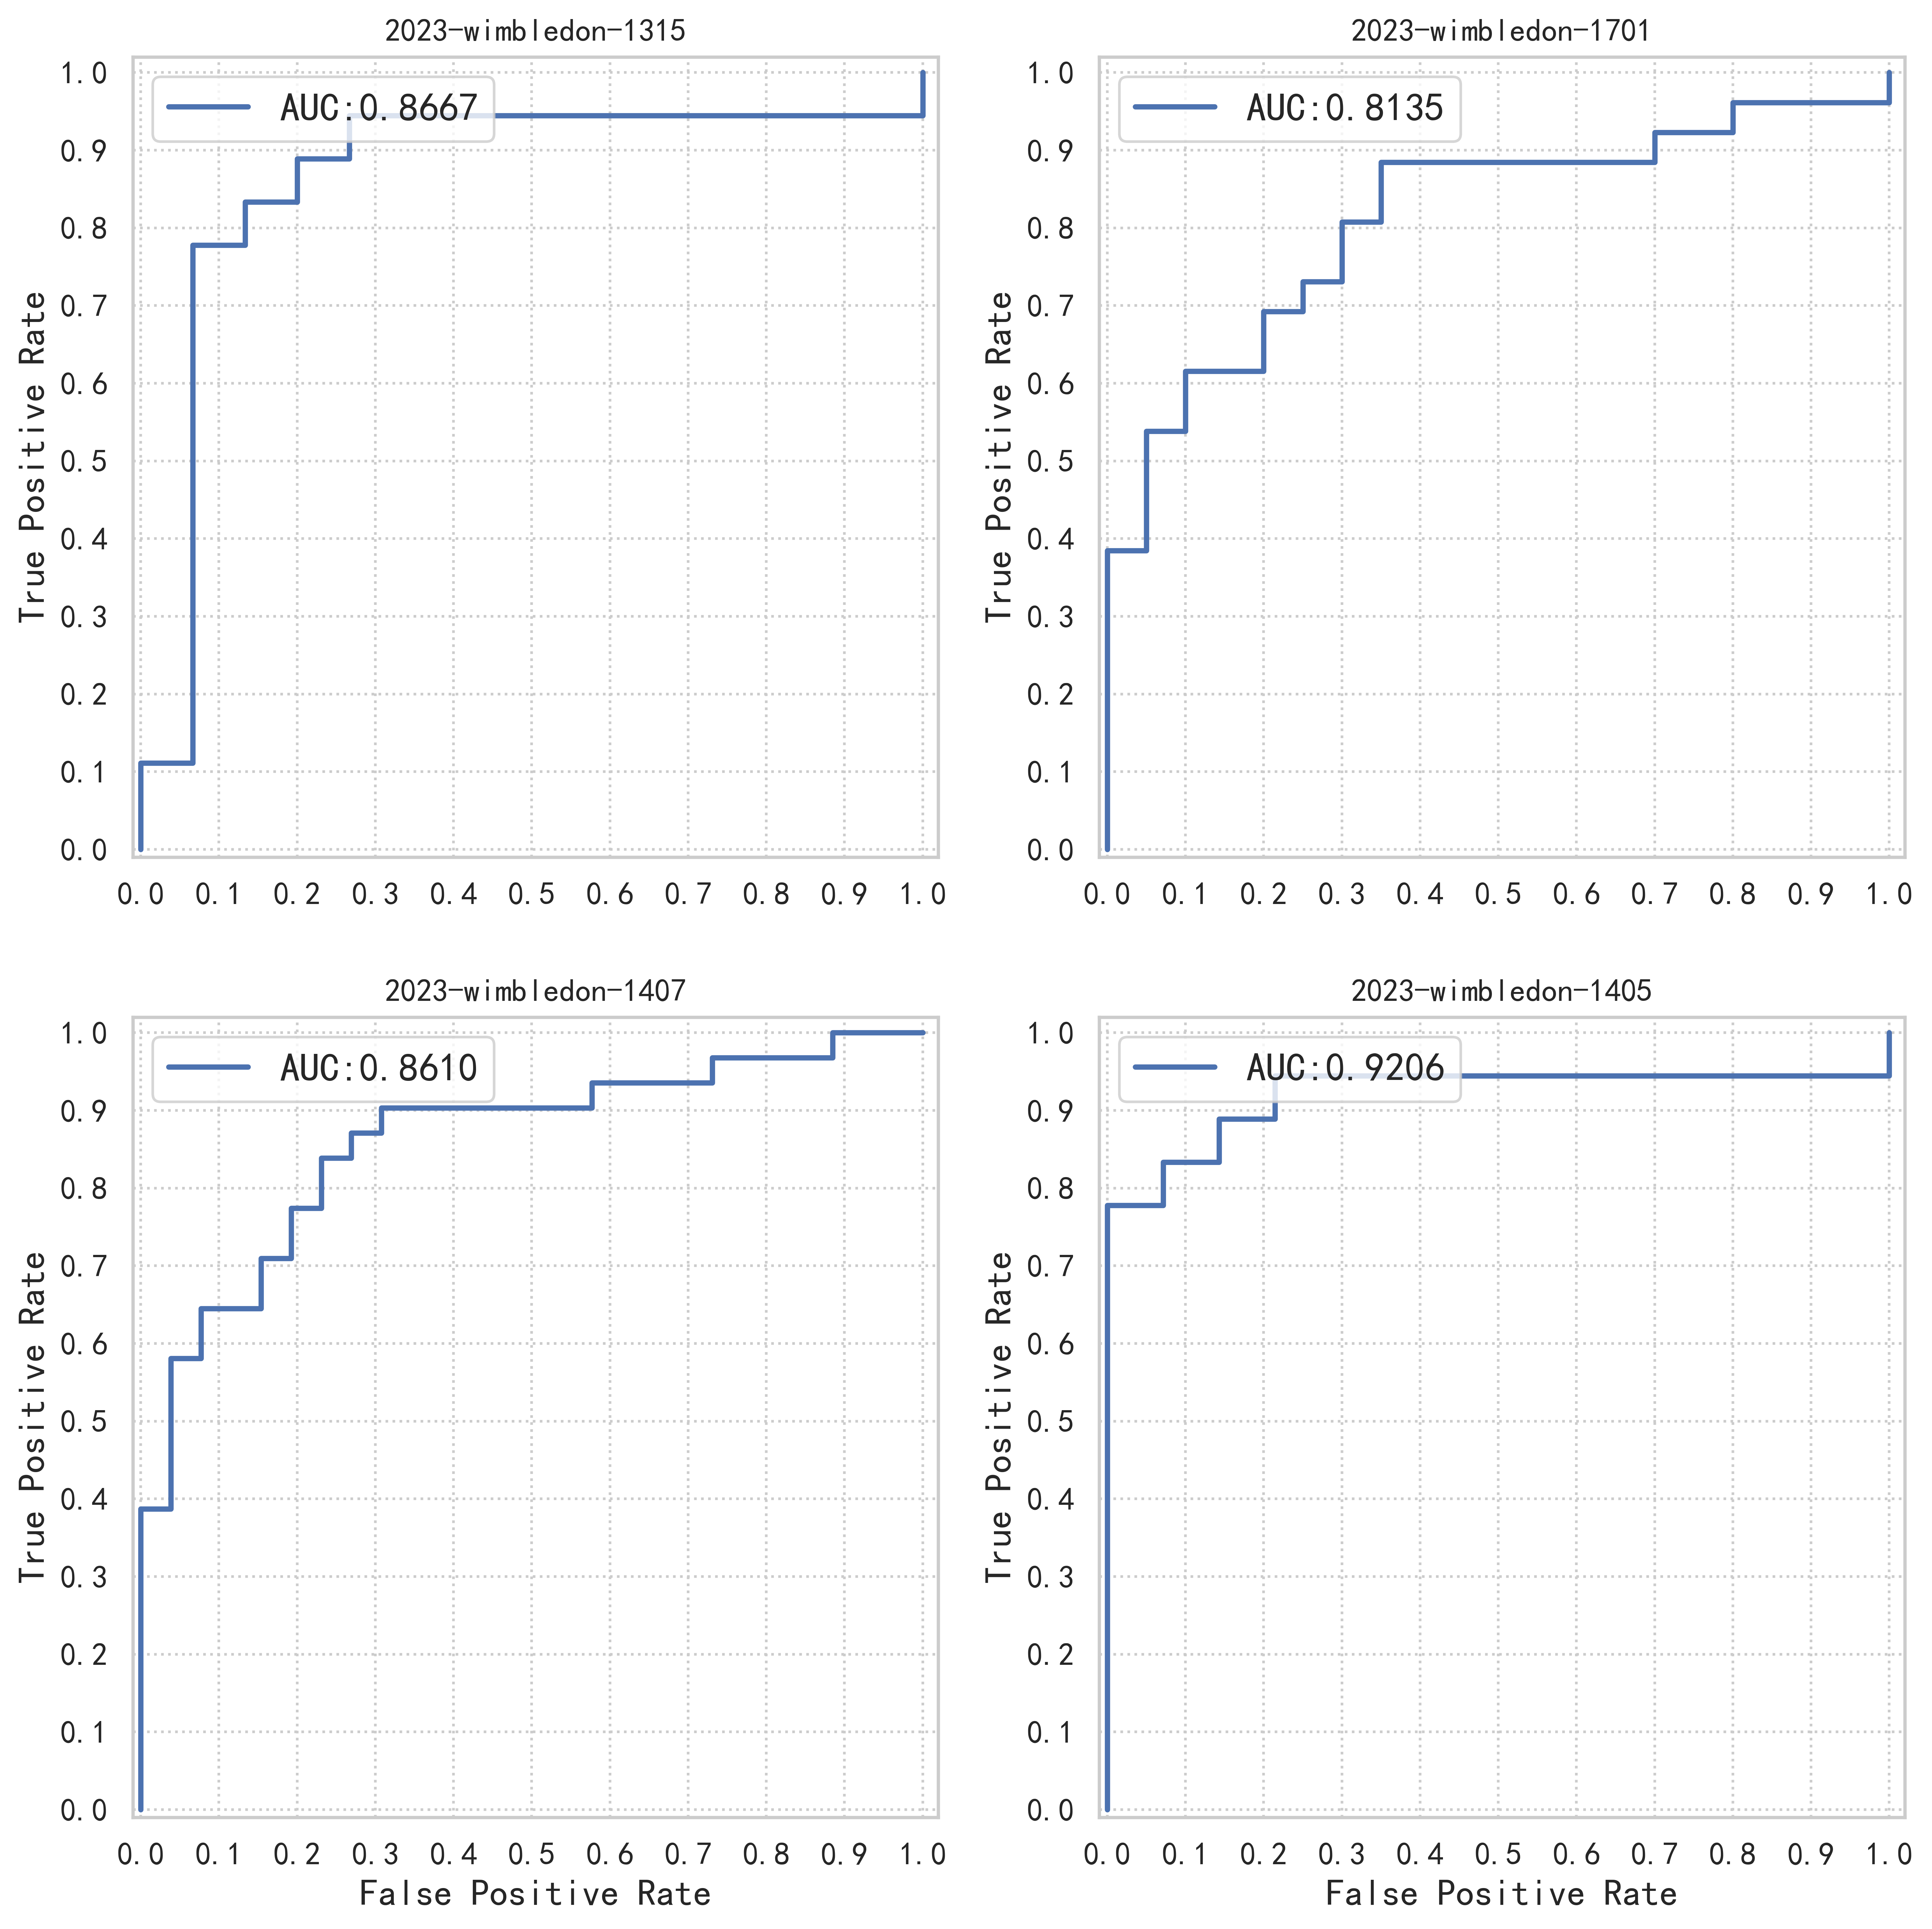
\includegraphics[width=0.55\textwidth]{reality.png}
\caption{reality}
\end{figure}

In response to this, this article believes that the indicator system actually has certain flaws. This comes from the fact that the model has no prior knowledge about the players. Therefore, when the two players first started competing, the model prediction was not accurate enough. As time goes by, because the model has obtained The situation of the game, for example, a player with relatively strong ability has a high probability that his game set and game scores are higher than those of a player with weak ability, so the model gradually becomes more accurate.

Therefore, for future model factors, one of the important points is the player's personal ability, which can generally be obtained through the player's performance in past games.

For example, we have expanded the indicator system to classify players' abilities according to this year's competition results, and use the indicators that each player deserves
Based on the total number of sets, the ability index of each player is obtained. Specifically, we use the total number of points scored by each player as a new independent variable to construct indicators of the player's personal ability and opponent's ability. Analyze relationships between players.

\begin{figure}[H]
      \centering
      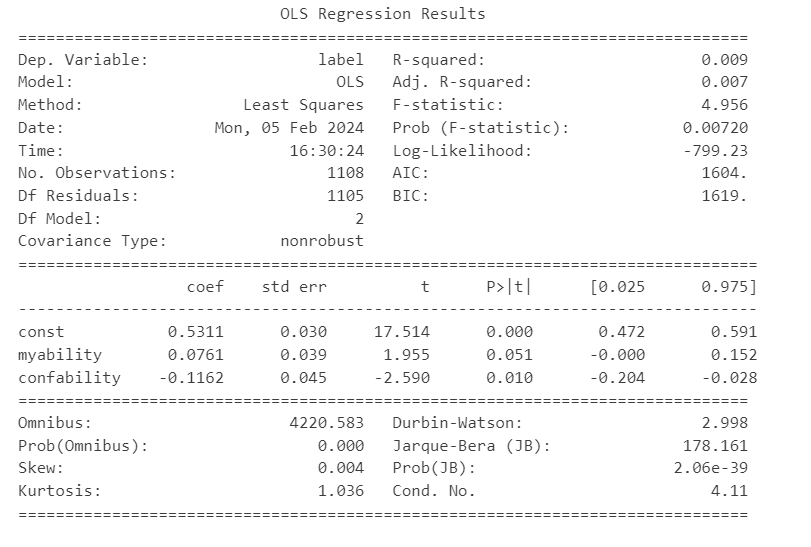
\includegraphics[width=0.6\textwidth]{logisticRegression2.png}
      \caption{The impact of player ability on winning}
\end{figure}

The results found that these two variables significantly affect the game winning situation. In particular, the opponent's ability is more important than personal ability.

\subsection{Generalization Assessment for Other Competitions}
\begin{enumerate}
      \item \textbf{Physical Condition and Fatigue Level:} The physical state of an athlete is a cornerstone of performance across all sports disciplines. Fatigue, both physical and mental, can drastically reduce an athlete's efficiency and reaction times. It is crucial to monitor an athlete's energy levels, recovery rate, and overall physical readiness. In games such as basketball, soccer, or swimming, the endurance and stamina dictated by an athlete's physical condition can be the deciding factor between victory and defeat.
      \item \textbf{Technical Skills:} The technical skill set of an athlete, which includes coordination, precision, and specific sport-related techniques, is a universal predictor of success. For instance, the precision in a tennis serve, the footwork in football, or the shooting accuracy in basketball, all reflect the athlete's technical proficiency. Developing these skills through rigorous practice is essential for an athlete to perform consistently under competitive pressure.
      \item \textbf{Psychological State and Momentum:} Athletes' mental state greatly influences their performance. Confidence, focus, and the ability to maintain composure can propel athletes to outperform their opponents. The concept of momentum, or the 'hot hand,' where success breeds further success, is seen in many sports. This psychological boost can lead to streaks of exceptional performance, as commonly observed in volleyball scoring runs or a boxer's domination in consecutive rounds.
\end{enumerate}

\subsection{Recommendations}
\begin{enumerate}
      \item \textbf{Real-time Mental Management:} Coaches should emphasize the management of a player's mental state during a match to capitalize on positive momentum. Techniques such as mindfulness, visualization, and breathing exercises can help athletes maintain focus, reduce anxiety, and enhance their in-game decision-making. A positive mental attitude can be the difference-maker in high-pressure situations, aiding players in executing their skills under stress and reversing negative trends during competition.
      \item \textbf{Technical Skill Development:} Enhancing a player's technical skills is vital for leveraging momentum. Coaches should focus on individualized skill drills that improve precision, accuracy, and execution under pressure. For example, a basketball player could work on free throws under simulated pressure conditions, or a soccer player might practice penalty kicks after intensive physical activity. Mastery of these skills enables athletes to seize moments of momentum during a game.
      \item \textbf{Tactical Strategy Adjustment:} Understanding momentum allows coaches to adjust strategies dynamically throughout a game. By recognizing when their team has the momentum, coaches can implement more aggressive tactics or when losing it, switch to conservative plays to regain control. Quick strategic shifts in response to momentum changes can outmaneuver opponents and turn the tide of a game.
\end{enumerate}
\section{Strength and Weakness}

\textbf{Strengths:}
\begin{enumerate}
      \item Comprehensive Consideration of Conditions:The model effectively utilizes data, taking into account factors such as athletes' physical fitness, technical skills, real-time mental state during competitions, and future variables. It considers a wide range of conditions for the competitors.
      \item High Generalizability and Applicability:Theoretically, this model can be applied not only to tennis matches but also to other competitions
      \item Objective Results:All outcomes of the model can be intuitively visualized and represented without being subject to personal bias.
      \item High Frequency:The model successfully predicts changes in athletes' momentum under different conditions, saving experts a significant amount of time in forecasting match situations.
      \item Dynamic Adaptation:As more input data is added, the accuracy of the model improves with ongoing adjustments.
      \item Simple to Understand:Despite including complex concepts such as machine learning models and quantitative data, the basic principles and operation of the model are understandable to everyone.
      \item Accuracy:By further optimizing the model, the accuracy of the data improved from 65.5\% to 71.4%. Moreover, the model with updating measures possesses the ability to self-correct, enhancing its accuracy.
      \item Innovative:The model employs 5-fold cross-validation, addressing the low precision issue inherent in binary logistic regression models.
      \item High Power Consumption and Inability for Real-time Analysis:The model requires substantial power, hindering its capacity for real-time analysis.
\end{enumerate}
\textbf{Weaknesses:}
\begin{enumerate}
      \item Relatively Unstable:Given that an athlete's momentum is heavily influenced by subjective factors, the model cannot achieve extremely high accuracy.
      \item Time-consuming: Due to the system's consideration of numerous factors, the model is complex and has lower computational efficiency.
\end{enumerate}

\section{Memo}
\begin{center}
      \textbf{Memo}
\end{center}
To: The tennis instructor\\
\ From: Team \#2417022\\
\ Date: February 5, 2024\\
\ Subject: The Predicting and Strategies for Dealing with Players' "Momentum"

Dear Sir/Madam,\\

At first,the tennis sport is born in 13 centuries in France.With the development of tennis sport,at the first modern Olympic Games in Athens in 1896,men's singles and doubles tennis were made official.By now, modern tennis was officially formed and quickly became popular in Europe and the United States, becoming a popular ball game.In the 2023 Wimbledon Gentlemen's final, the successive victories was lost by Novak Djokovic owing to a new Spanish player,Carlos Alcaraz.As tennis continues to evolve, there is a growing emphasis on the fluctuations in opponents' scores during tennis matches to explore the secret behind the tennis match,”momentum”.

To help with the endeavor to analyze the impact of momentum, we propose a model to predict the behaviour of the players following the processing the match, and provide the advice for coaches and players to let them know how to react the the events impacting the play during the matches.

Simply put, the model works in three steps:

1. Build a model to analyze the effect of players' fatigue level, individual technical skills, and psychological state during the game on the scoring of the game by processing the existing game data.

2. Use the data obtained in the first step to predict the change of "momentum" of different players in different time periods, and determine when to change players to favor the situation.

3. By adding future factors to the model, the model can be further analyzed and extended to increase the reliability of the model to predict the “momentum” of the players.

In the process, our team used the data provided to analyze the information reflected by the data and create the model.Moreover,we introduced the future factors to further improve the fit and reliability of the model, our model achieves a high degree of accuracy:71.4\%. Predicting the scoring of players by “momentum” in a match can be a daunting task, but our model can be very helpful to solve it.

\begin{center}
      \textbf{Results:}
\end{center}

Based on the modeling and analysis of the data, we got the following results:

1. Create a model to predict changes in a player's "momentum" during a game and the impact on game scoring.

2. Changes in "momentum" have an important and direct impact on game scoring during the game.

3. Other factors such as individual technical ability, running distance and other factors are important factors affecting the scoring of the "momentum" of the game.

4. The "momentum" and score of an unknown game can be inferred from the existing model and the model could update following the the addition of the data.

5. Further enhance model reliability by including future factors to further generalize model utility

\begin{center}
      \textbf{Strategies:}
\end{center}

On the basis of the above result, we can come up with recommendations for coaches and players to let them know how to solve the problem of lacking “momentum” in the processing of match:

\begin{center}
      \textbf{For coaches:}
\end{center}

1.Use modeling and switching players at the right time to keep your own team's in high "momentum" and let the situation tend to your own team.

2.Strengthen the players' physical strength, technical skills and so on through exercise to offset the decreasing of "momentum".

3.Analyzing game data after every game to know the situation of every player.

\begin{center}
      \textbf{For players:}
\end{center}

1.Train the psychological quality to meet the challenge of the loss of "momentum",such as losing the ball in one game.

2.Adjust psychology when loss score to let yourself have a better mindset to go on.

We hope this model can serve as a valuable tool to predict the scoring of the players in a better method.After all,it is the responsibility of each and every one of us to make the game of tennis grow in a more harmonious and healthy way.If there are any further Tasks or problems about this model,please contact us and we will spare no effort to explain and improve the model.

\ Yours Sincerely,
\ Team \#2417022

\section{Sensitivity Analysis}
We focus on classification thresholds, feature importance, and hyperparameter tuning to predict the sensitivity of a logistic regression mode in tennis match.

First,we find that adjusting the threshold from the default 0.5 showed significant impacts on model metrics like precision and recall. Optimal threshold finding, tailored to balance false positives and negatives, proved crucial for enhancing model accuracy.

Later,analysis revealed key features such as serve success rate and score differences as highly predictive. This highlights the potential for targeted feature engineering to improve model performance and interpretability.

Finally,systematic tuning of logistic regression parameters, including regularization strength, demonstrated their influence on model generalization and performance. Optimal settings were identified to improve accuracy and reduce overfitting.


\section{Conclusion}
In this paper, we have developed a model that enables coaches to predict the substantial impact of "momentum" during matches and better manage the overall flow of the game. Initially, we established indicators using the LOGISTIC method that may affect a player's momentum, such as fatigue levels, individual technical skills, and real-time mental state during matches. We then compared the reliability of various machine learning algorithms, including LGBM, XGBOOST, SVC, MLP, and LR, and selected the best-fitting LGBM algorithm as our model. This model was tested with datasets to obtain Pearson correlation coefficients and probability output values, which were analyzed to determine the correlation between these outputs and actual scores. 

Subsequently, a simple linear regression model was employed to speculate on the dynamic characteristics of player performance. To further enhance the model's reliability, we used data predicting single-game victories, which eliminated the high scoring rate's bias for the serving side, repeating the steps from the initial issue and ultimately selecting the most fitting support vector machine model to represent "momentum" fluctuations. Finally, we incorporated additional future factors to improve the model's reliability further and to extend its application for predicting player "momentum" in other competitions such as tournaments.

Over time, as more data becomes available, we can continually enhance the model's reliability by adding new factors and training data. Additionally, we have composed a memo for coaches to aid them in understanding changes in player "momentum" and mastering the overall dynamics of tennis matches.

\begin{thebibliography}{9}

    \item An Xin, Su Shiguang, Wang Tao, Xu Shuo, Huang Wenjiang, Zhang Ludai. \emph{Composite Support Vector Machine Method and Its Application in Spectral Analysis.} \emph{Spectroscopy and Spectral Analysis}, 2007, 8.

    \item Fan Zhiyin, Gou Xiaofeng, Qin Mingyue, Fan Qiang, Yu Jianle, Zhao Jianjun. \emph{Evaluation of Geological Hazard Susceptibility Based on Coupling Information Quantity Model and Logistic Regression Model.} Key Laboratory of Geological Hazards Prevention and Geological Environment Protection of Ministry of Education (Chengdu University of Technology), 2018.

    \item Lu Wencong, Chen Nianyi, Ye Chenzhou, Li Guozheng. \emph{Introduction to the Support Vector Machine Algorithm and Software ChemSVM.} Computer Chemistry Research Laboratory, Department of Chemistry, School of Science, Shanghai University, Institute of Image and Pattern Recognition, Shanghai Jiao Tong University, 2002, 11.

    \item Wu Lijun. \emph{Research on the Sustainable Development of Competitive Tennis in China} [D]. Shanxi University, 2010.

    \item Wei Zide, Wang Wenqin. \emph{Exploration of Tennis Introduction Teaching for Female Students in Ordinary Colleges and Universities.} \emph{Journal of Sports Science and Technology Literature Bulletin}, 2007, (02): 29-30+40.

    \item Yang Mianrong, Niu Liping. \emph{Feature Selection and Infrared Image Target Recognition Based on LGBM.} \emph{Proceedings of the College of Computer and Information Engineering, Xinxiang University}, College of Computer and Information Engineering, Henan Normal University, 2022, 4.

    \item Yang Xinhui. \emph{Machine Learning for Predicting Five-Year Survival Rate of Cancer Patients.} School of Mathematics and Statistics, Qingdao University, 2023, 12(5).

    \item Ye Hangjun, Bai Xuesheng, Xu Guangyou. \emph{Face Pose Determination Based on Support Vector Machine.} \emph{Journal of Tsinghua University (Science and Technology)}, 2003, 1: 67-70.

\end{thebibliography}



\section{Appendix}

\textbf{Data Preprocessing and standardization}
\begin{lstlisting}[caption={Data Preprocessing and standardization}, label=python-example]
from sklearn.preprocessing import MinMaxScaler
scaler = MinMaxScaler()
columns = dataset.columns[:-1]
scaler.fit(dataset[columns].values)
dataset[columns] = scaler.transform(dataset[columns].values)
dataset.to_excel('Standard_Training_Data.xlsx',index=False)
\end{lstlisting}

\textbf{Machine Learning Model: ccuracy, recall, precision, f1 and auc}
\begin{lstlisting}[caption={Machine Learning Model: ccuracy, recall, precision, f1 and auc}, label=python-example]
      def function(model):
          auc = round(cross_val_score(model,dataset[columns].values,dataset['label'].values, cv=5,scoring='roc_auc').mean(),2)
          acc = round(cross_val_score(model,dataset[columns].values,dataset['label'].values, cv=5,scoring='accuracy').mean(),2)
          recall = round(cross_val_score(model,dataset[columns].values,dataset['label'].values, cv=5,scoring='recall').mean(),2)
          precision = round(cross_val_score(model,dataset[columns].values,dataset['label'].values, cv=5,scoring='precision').mean(),2)
          f1 = round(cross_val_score(model,dataset[columns].values,dataset['label'].values, cv=5,scoring='f1').mean(),2)
          return acc,recall,precision,f1,auc

      model = LGBMClassifier(random_state=30,force_col_wise=True)
      print(f'LGBMClassifier acc,recall,precision,f1,auc :{function(model)}')
      model = XGBClassifier(random_state=50)
      print(f'XGBClassifier acc,recall,precision,f1,auc :{function(model)}')
      model = SVC(random_state=50)
      print(f'SVC acc,recall,precision,f1,auc :{function(model)}')
      model = MLPClassifier(random_state=60)
      print(f'MLPClassifier acc,recall,precision,f1,auc :{function(model)}')
      model = LogisticRegression(random_state=50)
      print(f'LogisticRegression acc,recall,precision,f1,auc :{function(model)}')
\end{lstlisting}

\textbf{Classic duel}
\begin{lstlisting}[caption={Classic duel}, label=python-example]
index = df[df.match_id=='2023-wimbledon-1701'].reset_index(drop=True).index
test = dataset.iloc[index]
train = dataset.drop(index,axis=0)
model = LGBMClassifier(random_state=30)

modelfit(train[columns].values,train['label'].values)
pred = model.predict_proba(test[columns].values)
pred = pd.DataFrame({'real_time_score':pred[:,1]})

match1 = pred.iloc[:45]
match2 = pred.iloc[45:126]
match3 = pred.iloc[126:195]
match4 = pred.iloc[195:259]
match5 = pred.iloc[259:]

plt.figure(figsize=(12, 6), dpi=80, facecolor='w')
plt.plot(match1.index,match1.values)
plt.plot(match2.index,match2.values)
plt.plot(match3.index,match3.values)
plt.plot(match4.index,match4.values)
plt.plot(match5.index,match5.values)

plt.xlabel("Points")
plt.ylabel("Performance")
plt.savefig('task1_image\\classic_duel_trend.png',dpi=500)
plt.show()
\end{lstlisting}

\textbf{Pearson coefficient}
\begin{lstlisting}[caption={Pearson coefficient}, label=python-example]
import scipy.stats as stats
# fit the model
model = LGBMClassifier(random_state=30)
model.fit(xtrain,ytrain)
 
pred = model.predict_proba(xvalid)[:,1]
# calculate Pearson's correlation
corr_coef, p_value = stats.pearsonr(pred, yvalid)
print("Pearson Correlation coefficient:", round(corr_coef,3))
print("p value:", p_value)
from statsmodels.regression.linear_model import OLS

import statsmodels.api as sm

y = yvalid
x = pred
X = sm.add_constant(x)
model = OLS(y,X,fit_intercept=True).fit()
print(model.summary())
\end{lstlisting}
\end{document}